\documentclass{beamer}

\usetheme{Boadilla}

\usepackage[utf8]{inputenc}
\usepackage[francais]{babel}
\usepackage{multicol} % itemize sur plusieurs colonnes
\usepackage{tikz} % pour tracer des figures
\usepackage{subfig} % pour mettre images à côté
\setcounter{tocdepth}{1} % afficher que les sections dans le sommaire

\hypersetup{ % couleur des liens
    colorlinks=true,
    linkcolor=blue,
    filecolor=black,      
    urlcolor=blue,
}

\AtBeginSection[] % faire apparaître le sommaire avant chaque nouvelle section
{
  \begin{frame}
    \frametitle{Sommaire}
    \tableofcontents[currentsection]
  \end{frame}
}

\newif\ifplacelogo %Booléen pour placer ou non le logo
\placelogotrue %Initialisation booléen à 'True'
\logo{\ifplacelogo
\includegraphics[height=5mm]{Images/logoINSA.png}\fi} %Initialisation du logo (fonction du booléen)

\title{Filtre de Canny-Deriche}
\author[AM \--- TD]{ABOUZAID Mehdi \\ TOOMEY Damien}
\institute[INSA Rouen]{INSA \--- Institut National des Sciences Appliquées de Rouen}
\date{\today}

\begin{document}

\begin{frame}
\titlepage
\end{frame}

\placelogofalse
\begin{frame}
\frametitle{Sommaire} 
\tableofcontents
\end{frame}	

\section{Introduction}
\begin{frame}
\frametitle{Introduction} 
\begin{itemize}
	\item[•] Détection de contours $\rightarrow$ réduction d'information $\rightarrow$ stockage réduit
	\item[•] Rachid Deriche, 1987
	\item[•] Amélioration du filtre de Canny
\end{itemize}

\centerline{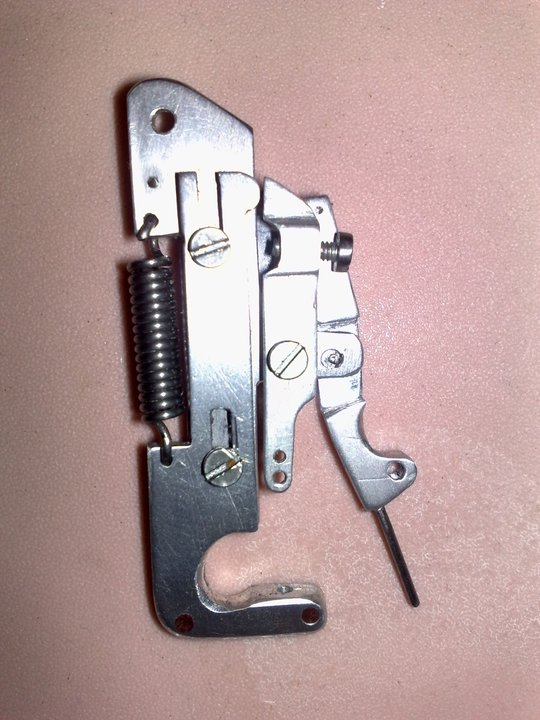
\includegraphics[height=5cm]{Images/intro_originale} \hspace{0.5cm} 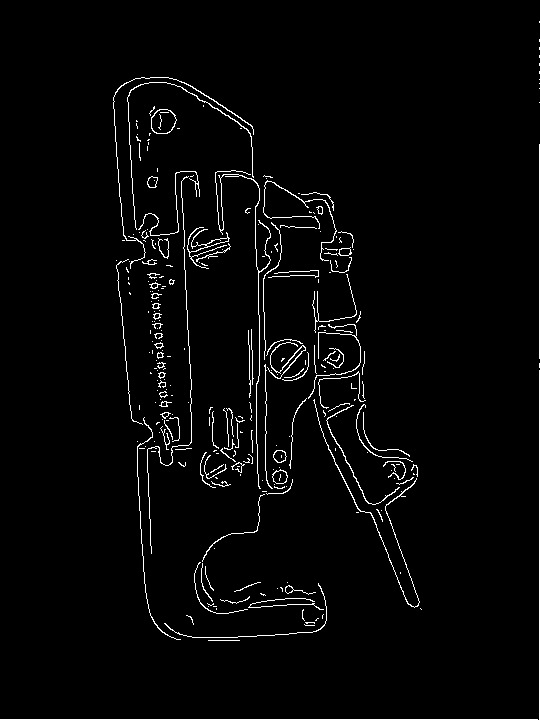
\includegraphics[height=5cm]{Images/intro_filtree}}

\begin{tikzpicture}[overlay]
	\node(a)[anchor=center, xshift=6cm, yshift=0.1cm]{\centerline{$ \alpha = 0.8 $, $ \text{\emph{Smin}} = 26 $, $ \text{\emph{Smin}}= 41 $}};
\end{tikzpicture}
\end{frame}	

\section{Description du filtre}
\begin{frame}
\frametitle{Similitudes avec le filtre de Canny} 

\begin{block}{Méthode}
Détection de contours en 4 étapes, comme le filtre de Canny : 
\begin{itemize}
\item[\textbf{1}] Gradients et lissage (réduction du bruit)
\item[\textbf{2}] Norme du gradient et direction du gradient
\item[\textbf{3}] Suppression des non-maxima locaux
\item[\textbf{4}] Seuillage par hystérésis
\end{itemize}
\end{block}
\end{frame}	


%\begin{frame}
%\frametitle{La détection de contours en 4 étapes} 
%
%\hspace{1.5cm} 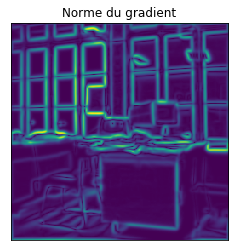
\includegraphics[height=4cm]{Images/Python/norme_gradient} \hspace{1cm} 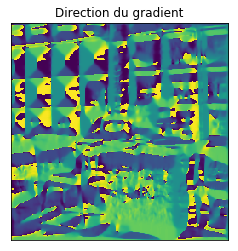
\includegraphics[height=4cm]{Images/Python/direction_gradient} \\
%\hspace{1.2cm} 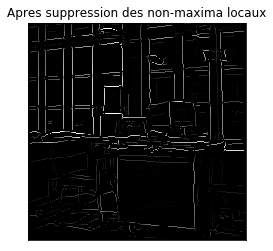
\includegraphics[height=4cm]{Images/Python/non_maxima} \hspace{0.8cm} 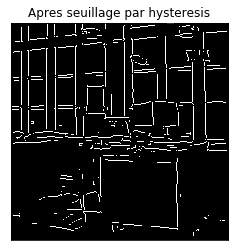
\includegraphics[height=4cm]{Images/Python/seuillage_hysteresis}
%\end{frame}	

\begin{frame}
\frametitle{Critères de détection optimale des contours} 

\begin{alertblock}{Remarque}
Dans le filtre de Deriche, on retrouve également les mêmes critères de détection optimale des contours que le filtre de Canny 
\end{alertblock}

\begin{itemize}
\item[\textbf{A}] \textbf{Bonne détection} : faible taux d'erreur dans la signalisation des contours
\item[\textbf{B}] \textbf{Bonne localisation} : les points détectés comme contours doivent être aussi proches que possible des contours réels
\item[\textbf{C}] \textbf{Clarté de la réponse} : un point du contour ne doit être détecté qu'un seule fois par le filtre \\
\end{itemize}

A chaque critère (\textbf{A},\textbf{B},\textbf{C}) est associé une formule mathématique. La maximisation de ces trois critères conduit à la résolution de l'équation différentielle dont la solution est l'opérateur $ f $.

\end{frame}

\begin{frame}
\frametitle{Différences par rapport au filtre de Canny}
La principale différence se trouve dans l'implémentation des deux premières étapes de l'algorithme :
\begin{itemize}
\item[\textbf{1}] Gradients et lissage (réduction du bruit)
\item[\textbf{2}] Norme du gradient et direction du gradient
\end{itemize}

\centerline{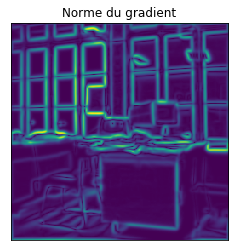
\includegraphics[height=3.5cm]{Images/Python/norme_gradient} 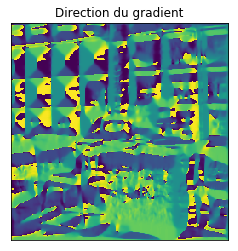
\includegraphics[height=3.5cm]{Images/Python/direction_gradient}}

Contrairement au filtre de Canny, le détecteur de contours de Deriche utilise \textbf{un filtre RII (Réponse Impulsionnelle Infinie)} au lieu d'un filtre RIF (Réponse Impulsionnelle Finie)

\end{frame}

\begin{frame}
\frametitle{}

\begin{block}{Equation différentielle}
\centerline {$ 2 \cdot f(x) - 2 \cdot \lambda_1 \cdot f''(x) + 2 \cdot \lambda_2 \cdot f''''(x) + \lambda_3 = 0$} 
\end{block}

\begin{block}{Canny : filtre RIF} 
Conditions initiales :
$ f(0)=0, f(W)=0, f'(0)=S$ et $f'(W)=0 $

Solution générale sur $ [-W,W] $ : \\

\centerline{$ f(x) = a_1 \cdot e^{\alpha \cdot x} \cdot sin(\omega \cdot x) + a_2 \cdot e^{\alpha \cdot x} \cdot cos(\omega \cdot x) + a_3 \cdot e^{-\alpha \cdot x} \cdot sin(\omega \cdot x) + $} 
\centerline{$ a_4 \cdot e^{-\alpha x} \cdot cos(\omega \cdot x) + C $} 
\end{block}

\begin{block}{Deriche : filtre RII} 
Conditions initiales : 
$ f(0)=0, f(+ \infty)=0, f'(0)=S$ et $f'(+ \infty)=0 $

Solution générale sur $ \rm I\!R $ : \\
\centerline{$f(x)= -c \cdot e^{-\alpha \cdot |x|} \cdot sin(\omega \cdot x)$}
\end{block}

On peut observer que la solution obtenue à l'aide du filtre RII pour le détecteur de contours de Deriche est plus simple en plus d'améliorer les résultats de détection.

\end{frame}

\begin{frame}
\frametitle{Avantage du filtre RII de Deriche}
Adaptation aux caractéristiques de l'image en modifiant seulement les deux paramètres $ (\alpha, \omega) \in \rm I\!R^+ $, sans impacter le temps d'exécution.
\begin{itemize}
\item[•] Si la valeur de $ \alpha $ est petite (généralement entre $ 0.25 $ et $ 0.5 $), la détection est meilleure.
\item[•] Si la valeur de $ \alpha $ est grande (entre 2 et 3), la localisation des contours est meilleure.
\end{itemize}
\noindent
C'est pourquoi, dans la plupart des cas, il est recommandé de fixer la valeur de $ \alpha $ à 1.\\
\vspace{0.2cm}
\centerline{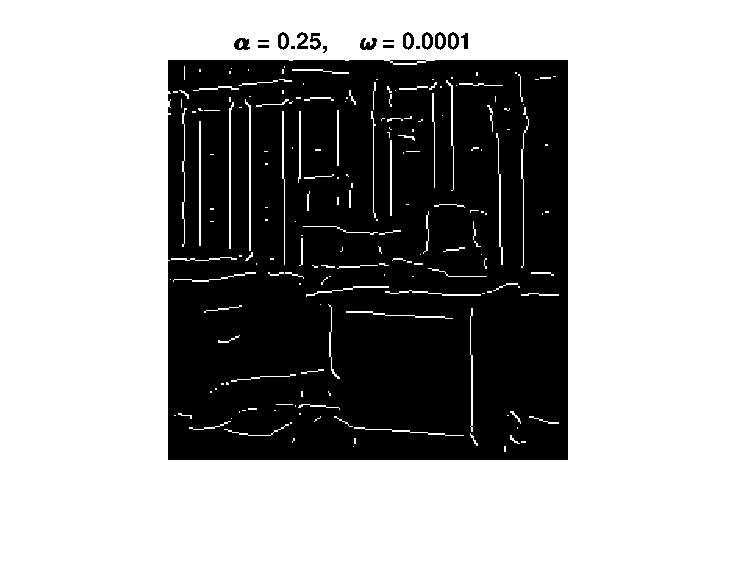
\includegraphics[trim = 3cm 0cm 3cm 0cm, clip, height=5cm]{Images/alpha025}
\hspace{0.2cm} 
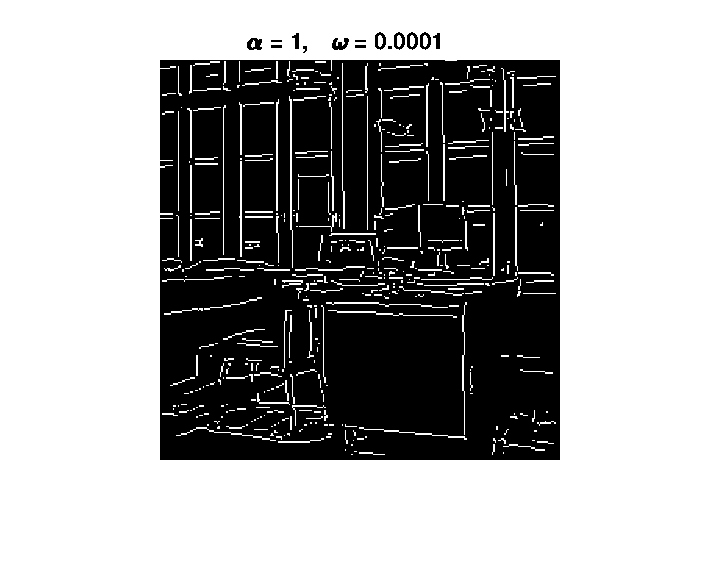
\includegraphics[trim = 3cm 0cm 3cm 0cm, clip, height=5cm]{Images/alpha1} \hspace{0.2cm} 
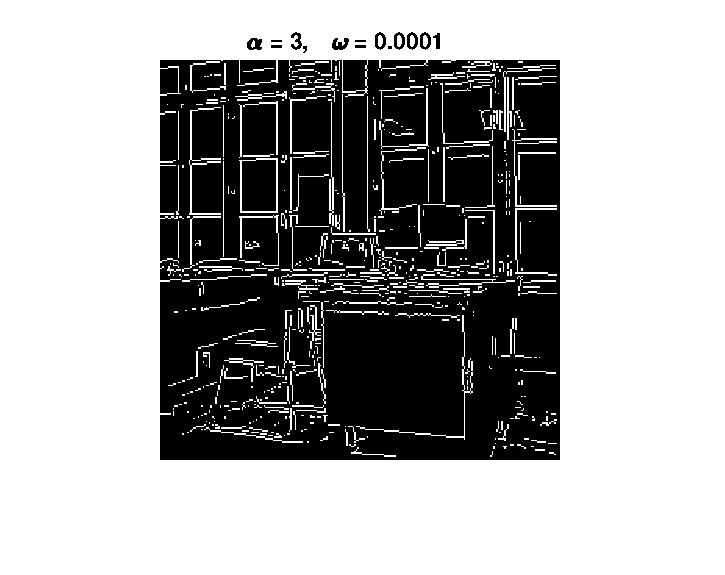
\includegraphics[trim = 3cm 0cm 3cm 0cm, clip, height=5cm]{Images/alpha3} \hspace{0.2cm}}

\end{frame}

\section{Modélisation mathématique}\label{modelisation_mathematique}

\begin{frame}
\frametitle{Cas mono-dimensionnel}

\begin{block}{Deux détecteurs de contours optimaux de réponse impulsionnelle :}
$ \hskip 9.7 em f(x) = -c \cdot e^{\alpha \cdot |x|} \cdot sin(\omega \cdot x) $ \\
$ \hskip 9.7 em g(x) = -c \cdot x \cdot e^{\alpha \cdot |x|} $
\end{block}

\begin{alertblock}{Remarque}
Les résultats de détection de contours sont améliorés en utilisant $ g(x) $ au lieu de $ f(x) $. \\
Avec $ g(x) $, le filtre ne dépend que de $ \alpha $ et non plus de $ \omega $.
\end{alertblock}

\begin{block}{Réponse impulsionnelle $ h(n) $ (fonction de lissage)}
$ \hskip 2 em h(n) $ correspond à l’intégrale $ h(x) $ de $ f(x) $ avec $ n \in \mathbb{Z}, \; x \in \rm I\!R $

\[ h(n) = (c_1 \cdot sin(\omega \cdot |n|) + c_2 \cdot cos(\omega \cdot |n|)) \cdot e^{-\alpha \cdot |n|} \]
\end{block}
\end{frame}

\begin{frame}
\frametitle{Coefficients du filtre}

\begin{alertblock}{Remarque}
La forme du filtre est déterminée par $ (\alpha, \omega) \in \rm I\!R^+ $. \\
On choisit ces deux paramètres en fonction de nos données. \\
\end{alertblock}

\[ \left\{\begin{array}{ll}
c= \frac{1-2 \cdot e^{-\alpha} \cdot cos(\omega) + e^{-2 \cdot \alpha}}{e^{-\alpha} \cdot sin(\omega)} \\
c_1 = \frac{k \cdot \alpha}{\alpha^2 + \omega^2} \\
c_2 = \frac{k \cdot \omega}{\alpha^2 + \omega^2} \\
b_1 = -2 \cdot e^{-\alpha} \cdot cos(\omega) \\
b_2 = e^{-2 \cdot \alpha}
\end{array}\right.
\quad
\left\{\begin{array}{ll}
a = -c \cdot e^{-\alpha} \cdot sin(\omega) \\
a_0 = c_2 \\
a_1 = (-c_2 \cdot cos(\omega) + c_1 \cdot sin(\omega)) \cdot e^{-\alpha} \\
a_2 = a_1 - c_2 \cdot b_1 \\
a_3 = -c_2 \cdot b_2 \\
\end{array}\right. \]

\[ k = \frac{(1-2 \cdot e^{-\alpha} \cdot cos(\omega) + e^{-2 \cdot \alpha}) \cdot (\alpha^2 + \omega^2)}{2 \cdot \alpha \cdot e^{-\alpha} \cdot sin(\omega) + \omega - \omega \cdot e^{-2 \cdot \alpha}} \]
\end{frame}

\begin{frame}
\frametitle{Cas bi-dimensionnel}

\begin{block}{Réponse impulsionnelle $ f(x,y) $}
\begin{align*}
& f(x,y) = -\frac{c \cdot k}{\alpha^2 + \omega^2} \cdot e^{- \alpha \cdot (|x| + |y|)} \cdot \textbf{[} sin(\omega \cdot x) \cdot (\alpha \cdot sin(\omega \cdot |y|) + \\
& \omega \cdot cos(\omega \cdot |y|)) + sin(\omega \cdot y) \cdot (\alpha \cdot sin(\omega \cdot |x|) + \omega \cdot cos(\omega \cdot |x|)) \textbf{]} \\
& \\
&  f(x,y) = \underbrace{f(x) \cdot h(y)}_{X} + \underbrace{h(x) \cdot f(y)}_{Y} \qquad \text{avec} \; (x,y) \in \rm I\!R^2 \\
\end{align*}
\end{block}

\begin{alertblock}{Remarque}
Le filtre est donc séparable en deux masques X et Y.
\end{alertblock}

\end{frame}

\begin{frame}
\vspace{0.8cm}
\hspace{-0.3cm}
\centerline{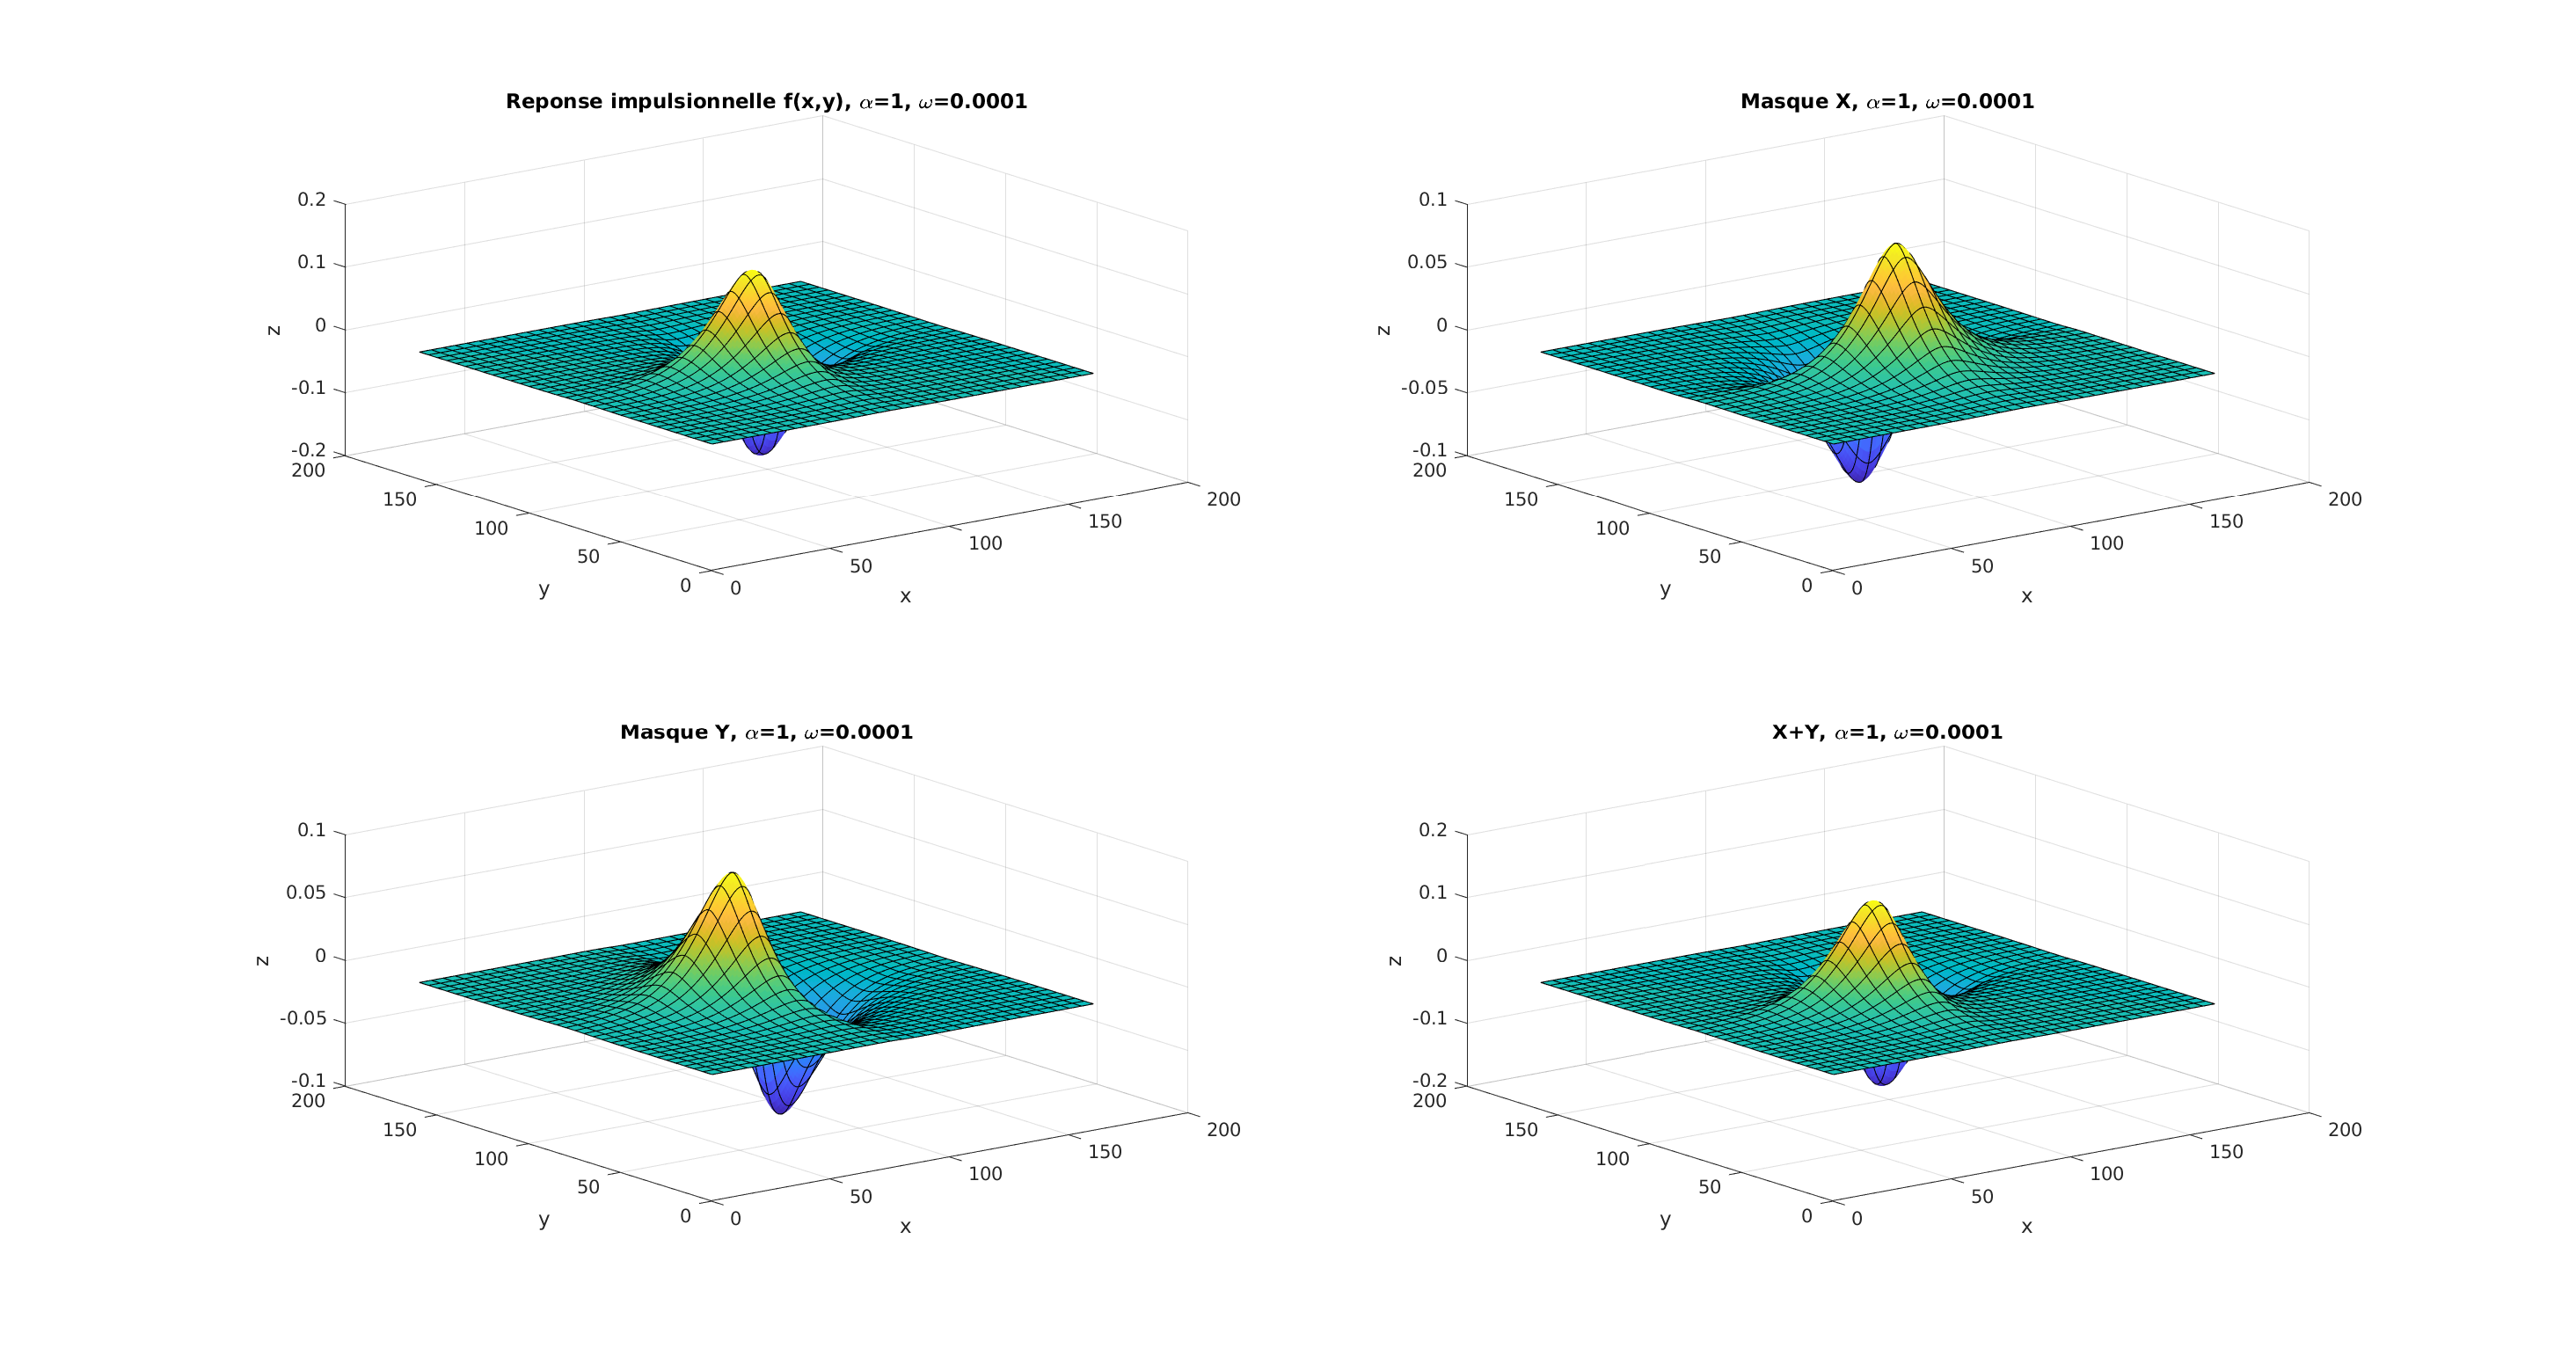
\includegraphics[width=15cm]{Images/Matlab/ResultatsConvolutions/f_X_Y}}


\end{frame}

\section{Explication de l'implémentation (cas 2D)}
\begin{frame}
\frametitle{Etape 1/4 : Gradients selon x et y et lissage (\textbf{récursif})}

\begin{exampleblock}{Gradient \textcolor{red}{selon x}}
$ Y^+(i,j)=I(i,j-1)-b_1 \cdot Y^+(i,j-1)-b_2 \cdot Y^+(i,j-2) $ \\
$ \quad j=1,...,NCL \quad i=1,...,NLG $ \\
\vspace{0.3cm}
$ Y^-(i,j)=I(i,j+1)-b_1 \cdot Y^-(i,j+1) - b_2 \cdot Y^-(i,j+2) $ \\
$ \quad j=NCL,...,1 \quad i= 1,...,NLG $ \\
\vspace{0.3cm}
$ S(i,j)=a \cdot (Y^+(i,j)-Y^-(i,j)) \quad j=1,...,NCL \quad i=1,...,NLG $
\end{exampleblock}

\begin{exampleblock}{Lissage}
$ R^+(i,j)=a_0 \cdot S(i,j) + a_1 \cdot S(i-1,j) - b_1 \cdot R^+(i-1,j) - b_2 \cdot R^+(i-2,j) $ \\
$ i=1,...,NLG \quad j=1,...,NCL $ \\
\vspace{0.3cm}
$ R^-(i,j) = a_2 \cdot S(i+1,j) + a_3 \cdot S(i+2,j) - b_1 \cdot R^-(i+1,j) - b_2 \cdot R^-(i+2,j) $ \\
$ i=NLG,...,1 \quad j=1,...,NCL $ \\
\vspace{0.3cm}
$ R(i,j)=R^-(i,j) + R^+(i,j) \quad i=1,...,NLG \quad j=1,...,NCL $
\end{exampleblock}

\end{frame}

\begin{frame}

\frametitle{Etape 1/4 : Gradient selon x et lissage (\textbf{convolutions})}

\begin{figure}[H]
%\caption{}
    \begin{tikzpicture}[overlay]
    \node(a)[anchor=center, xshift=-4cm, yshift=0.3cm]{\centerline{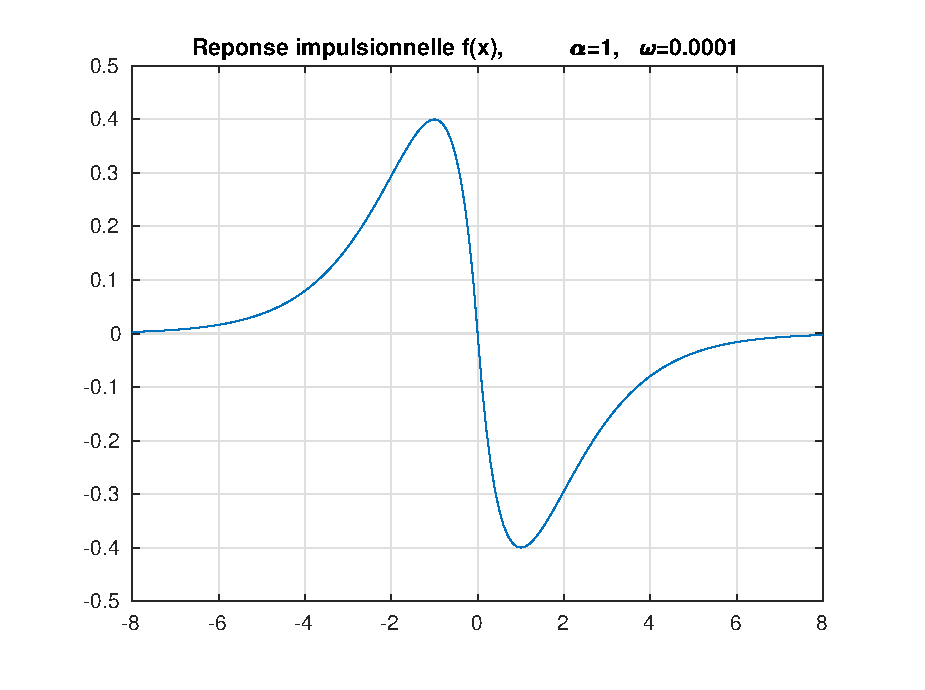
\includegraphics[width=0.43\textwidth]{Images/Matlab/ResultatsConvolutions/fx}}};
	\node(a)[anchor=center, xshift=-4cm, yshift=-4cm]{\centerline{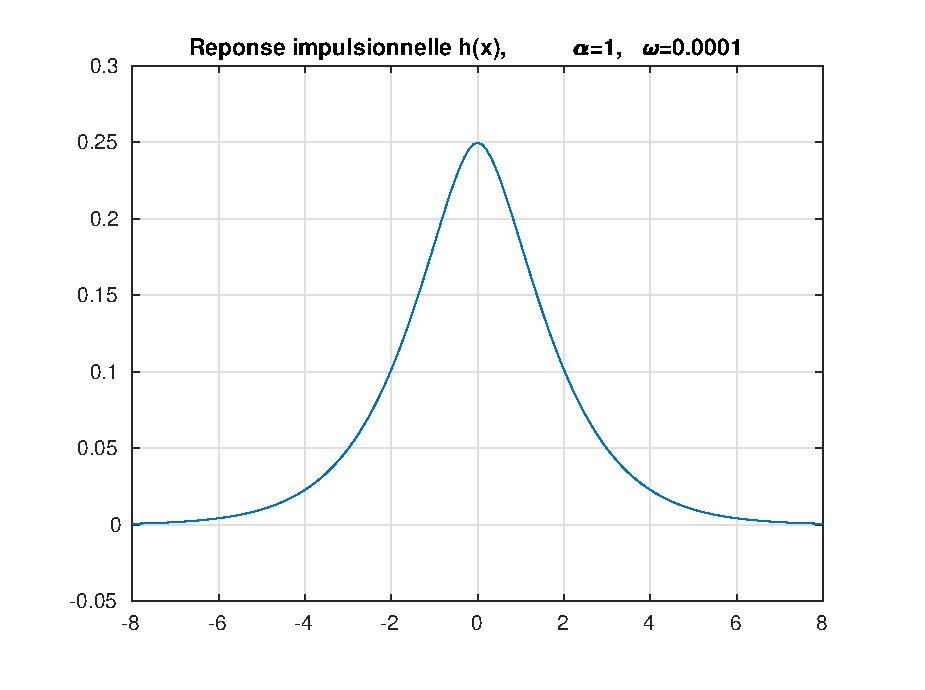
\includegraphics[width=0.43\textwidth]{Images/Matlab/ResultatsConvolutions/hx}}};
    \end{tikzpicture}    	
\end{figure}

$ \hskip 11 em \mathcal{I} = \begin{pmatrix}
i & i & i & i & i & i \\
i & i & i & i & i & i \\
i & i & i & i & i & i \\
i & i & i & i & i & i \\
i & i & i & i & i & i \\
i & i & i & i & i & i \\
\end{pmatrix} $


\begin{tikzpicture}[scale=3,cap=round,>=latex, overlay]
	\draw[->] (1.65cm,1.1cm) -- (2.65cm,1.1cm) node[midway,above,fill=none] {$ f(n) $ (gradient selon x)};
	\draw[->] (2.8cm,0.95cm) -- (2.8cm,0.05cm) node[midway,right,fill=none] {$ h(n) $ (lissage)};
	\node(a)[anchor=center, xshift=6cm, yshift=-0.7cm]{\centerline{$ n \in  [\![-N \cdot P;N \cdot P]\!] $}};
	\node(a)[anchor=center, xshift=7.15cm, yshift=-1.2cm]{\centerline{N : nombre de lignes dans l'image}};
	\node(a)[anchor=center, xshift=7.35cm, yshift=-1.7cm]{\centerline{P : nombre de colonnes dans l'image}};		
\end{tikzpicture}

\end{frame}

\begin{frame}

\frametitle{Etape 1/4 : Gradient selon y et lissage (\textbf{convolutions})}

\begin{figure}[H]
%\caption{}
    \begin{tikzpicture}[overlay]
    \node(a)[anchor=center, xshift=-4cm, yshift=0.3cm]{\centerline{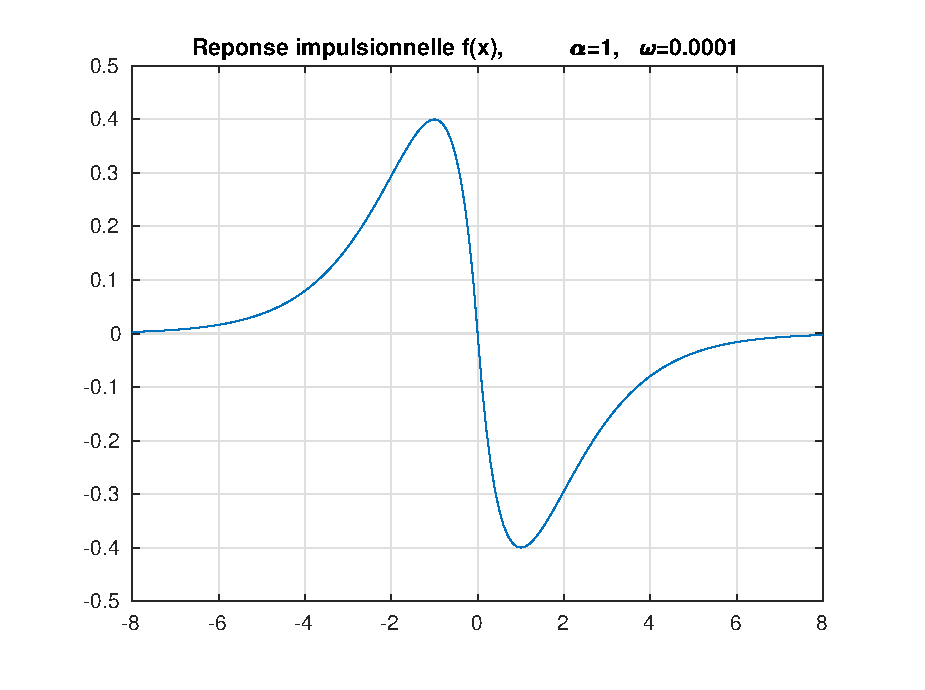
\includegraphics[width=0.43\textwidth]{Images/Matlab/ResultatsConvolutions/fx}}};
	\node(a)[anchor=center, xshift=-4cm, yshift=-4cm]{\centerline{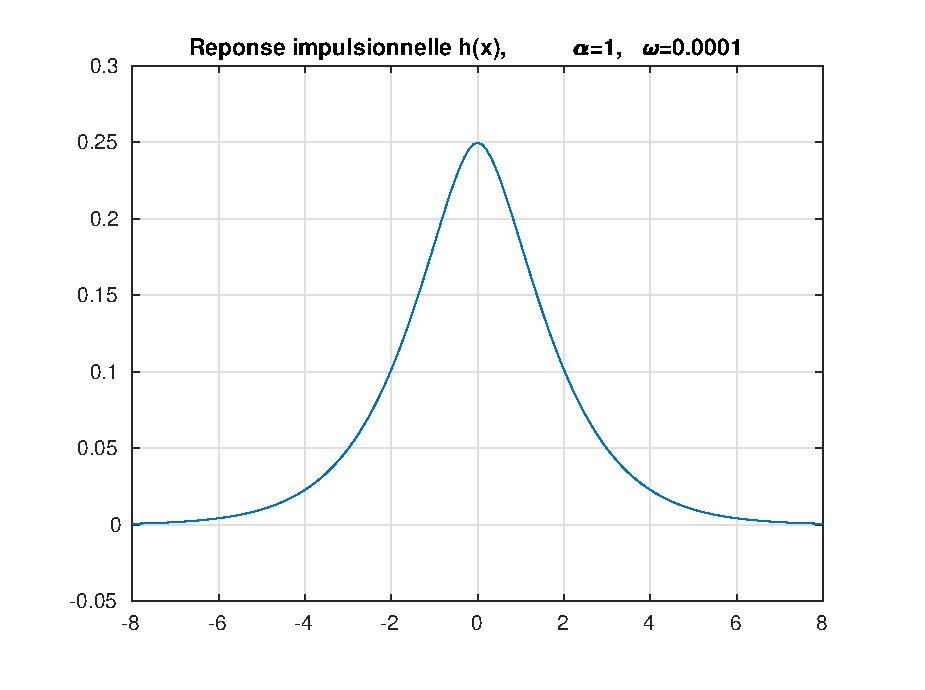
\includegraphics[width=0.43\textwidth]{Images/Matlab/ResultatsConvolutions/hx}}};
    \end{tikzpicture}    	
\end{figure}

$ \hskip 11 em \mathcal{I} = \begin{pmatrix}
i & i & i & i & i & i \\
i & i & i & i & i & i \\
i & i & i & i & i & i \\
i & i & i & i & i & i \\
i & i & i & i & i & i \\
i & i & i & i & i & i \\
\end{pmatrix} $

\begin{tikzpicture}[scale=3,cap=round,>=latex, overlay]
	\draw[->] (1.65cm,1.1cm) -- (2.65cm,1.1cm) node[midway,above,fill=none] {$ h(n) $ (lissage)}; 	
	\draw[->] (2.8cm,0.95cm) -- (2.8cm,0.05cm) node[midway,right,fill=none] {$ f(n) $ (gradient selon y)};
	\node(a)[anchor=center, xshift=6cm, yshift=-0.7cm]{\centerline{$ n \in  [\![-N \cdot P;N \cdot P]\!] $}};
	\node(a)[anchor=center, xshift=7.15cm, yshift=-1.2cm]{\centerline{N : nombre de lignes dans l'image}};
	\node(a)[anchor=center, xshift=7.35cm, yshift=-1.7cm]{\centerline{P : nombre de colonnes dans l'image}};	
\end{tikzpicture}
\end{frame}

\begin{frame}
\frametitle{Etape 2/4 : Norme du gradient et direction du gradient}

\begin{block}{Norme du gradient}
\[ A(m,n)=\sqrt{r(m,n)^2 + s(m,n)^2)} \]

\[ \text{avec }\left\{\begin{array}{ll}
r \; \text{gradient selon x} \\
s \; \text{gradient selon y}
\end{array}\right. \]
\end{block}

\begin{block}{Direction du gradient}
\[ \text{\emph{arg}} = arctan(\frac{s(m,n)}{r(m,n)}) \]
\end{block}

\end{frame}

\section{Suppression des non-maxima locaux}

\begin{frame}
\frametitle{Etape 3/4 : Suppression des non-maxima locaux}

\begin{block}{Définition}
Méthode appliquée sur la norme du gradient qui permet d'affiner les contours
\end{block}

\begin{block}{Méthode}
Mettre à 0 les pixels qui ne constituent pas un contour. \\
Un pixel de la norme du gradient est considéré comme contour s'il forme un maximum local dans la direction du gradient.
\end{block}

\end{frame}

\begin{frame}
\frametitle{Etape 3/4 : Suppression des non-maxima locaux}

\vspace{1.7cm}
\begin{center}
% http://www.texample.net/tikz/examples/unit-circle/
\begin{tikzpicture}[scale=2.7,cap=round,>=latex, overlay]

	% draw the coordinates
	\draw[->] (-1.5cm,0cm) -- (1.5cm,0cm) node[right,fill=white] {$x$};
	\draw[->] (0cm,0cm) -- (0cm,1.5cm) node[above,fill=white] {$y$};
	
	\foreach \x in {0,22.5,...,180} {
		  % draw each angle in degrees
		  \draw (\x:1.2cm) node[fill=white] {$\x^\circ$};
		  % lines from center to point
		  \draw[gray] (0cm,0cm) -- (\x:1cm);
		  % dots at each point
		  \filldraw[black] (\x:1cm) circle(0.4pt);
		  
	}
	
	\begin{scope}
	{\only<2,3>{
		\clip (-1.5,0) rectangle (1.5,1.5);\clip (-1.5,0) rectangle (1.5,1.5);
	}}
	\foreach \x in {-22.5,-45,...,-135} {
		  % lines from center to point
		  \draw[gray] (0cm,0cm) -- (\x:1cm);
		  % dots at each point
		  \filldraw[black] (\x:1cm) circle(0.4pt);
		  % draw each angle in degrees
		  \draw (\x:1.2cm) node[fill=none] {$\x^\circ$};
	}
	
	\foreach \x in {-157.5} {
		  % lines from center to point
		  \draw[gray] (0cm,0cm) -- (\x:1cm);
		  % dots at each point
		  \filldraw[black] (\x:1cm) circle(0.4pt);
		  % draw each angle in degrees
		  \draw (\x:1.26cm) node[fill=none] {$\x^\circ$};
	}
	
		% draw unit circle
		\draw[thick] (0cm,0cm) circle(1cm);	
	\end{scope}
	
	{\only<3>{
	\draw (8.5:1.42cm) node[fill=white] {\textcolor{red}{\textbf{Classe 1}}};	
	\draw (45:1.5cm) node[fill=white] {\textcolor{blue}{\textbf{Classe 2}}};
	\draw (90:1.35cm) node[fill=white] {\textcolor{green}{\textbf{Classe 3}}};
	\draw (135:1.5cm) node[fill=white] {\textcolor{magenta}{\textbf{Classe 4}}};
	\draw (171.5:1.42cm) node[fill=white] {\textcolor{red}{\textbf{Classe 1}}};
	
	\foreach \x in {0,1,...,22.5} {
	  % lines from center to point
	  \draw[red] (0cm,0cm) -- (\x:1cm);
	}
	
	\foreach \x in {22.5,23.5,...,67.5} {
	  % lines from center to point
	  \draw[blue] (0cm,0cm) -- (\x:1cm);
	}
	
	\foreach \x in {67.5,68.5,...,112.5} {
	  % lines from center to point
	  \draw[green] (0cm,0cm) -- (\x:1cm);
	}
	  
	\foreach \x in {112.5,113.5,...,157.5} {
	  % lines from center to point
	  \draw[magenta] (0cm,0cm) -- (\x:1cm);
	}
	
	\foreach \x in {157.5,158.5,...,180} {
	  % lines from center to point
	  \draw[red] (0cm,0cm) -- (\x:1cm);
	}}}
\end{tikzpicture}
\end{center}
\end{frame}

\begin{frame}
\frametitle{Etape 3/4 : Suppression des non-maxima locaux}

\begin{center}
{\only<2>{\textcolor{red}{\textbf{Classe 1}} : $ \text{\emph{arg}} \in [0; 22.5[ $ ou $ \text{\emph{arg}} \in [157.5; 180] $}}


\end{center}
\begin{align*}
& \quad \textbf{Direction du gradient} \qquad \qquad \quad \textbf{Norme du gradient} \\
& \begin{pmatrix}
D & D & D & D & D & D \\
D & {\only<1>{D}}{\only<2>{\color{red}\textbf{D}}} & D & D & D & D \\
D & D & D & D & D & D \\
D & D & D & D & D & D \\
D & D & D & D & D & D \\
D & D & D & D & D & D \\
\end{pmatrix}
\qquad \quad
\begin{pmatrix}
N & N & N & N & N & N \\
{\only<1>{N}}{\only<2>{\color{orange}\textbf{N}}} & {\only<1>{N}}{\only<2>{\color{cyan}\textbf{N}}}  & {\only<1>{N}}{\only<2>{\color{orange}\textbf{N}}} & N & N & N \\
N & N & N & N & N & N \\
N & N & N & N & N & N \\
N & N & N & N & N & N \\
N & N & N & N & N & N \\
\end{pmatrix}
\end{align*}

{\only<2>{
\begin{center}
Si $ non $(\textbf{\textcolor{cyan}{N}} $ \; \geq \; max $(\textbf{\textcolor{orange}{N}}, \textbf{\textcolor{orange}{N}})) alors \textbf{\textcolor{cyan}{N}} $ \leftarrow \; 0 $
\end{center}
}}

\end{frame}

\begin{frame}
\frametitle{Etape 3/4 : Suppression des non-maxima locaux}

\begin{center}
\textcolor{blue}{\textbf{Classe 2}} : $ \text{\emph{arg}} \in [22.5; 67.5[ $
\end{center}

\begin{align*}
& \quad \textbf{Direction du gradient} \qquad \qquad \quad \textbf{Norme du gradient} \\
& \begin{pmatrix}
D & D & D & D & D & D \\
D & \textcolor{blue}{\textbf{D}} & D & D & D & D \\
D & D & D & D & D & D \\
D & D & D & D & D & D \\
D & D & D & D & D & D \\
D & D & D & D & D & D \\
\end{pmatrix}
\qquad \quad
\begin{pmatrix}
N & N & \textcolor{orange}{\textbf{N}} & N & N & N \\
N & \textcolor{cyan}{\textbf{N}} & N & N & N & N \\
\textcolor{orange}{\textbf{N}} & N & N & N & N & N \\
N & N & N & N & N & N \\
N & N & N & N & N & N \\
N & N & N & N & N & N \\
\end{pmatrix}
\end{align*}

\begin{center}
Si $ non $(\textbf{\textcolor{cyan}{N}} $ \; \geq \; max $(\textbf{\textcolor{orange}{N}}, \textbf{\textcolor{orange}{N}})) alors \textbf{\textcolor{cyan}{N}} $ \leftarrow \; 0 $
\end{center}
\end{frame}

\begin{frame}
\frametitle{Etape 3/4 : Suppression des non-maxima locaux}

\begin{center}
\textcolor{green}{\textbf{Classe 3}} : $ \text{\emph{arg}} \in [67.5; 112.5[ $
\end{center}

\begin{align*}
& \quad \textbf{Direction du gradient} \qquad \qquad \quad \textbf{Norme du gradient} \\
& \begin{pmatrix}
D & D & D & D & D & D \\
D & \textcolor{green}{\textbf{D}} & D & D & D & D \\
D & D & D & D & D & D \\
D & D & D & D & D & D \\
D & D & D & D & D & D \\
D & D & D & D & D & D \\
\end{pmatrix}
\qquad \quad
\begin{pmatrix}
N & \textcolor{orange}{\textbf{N}} & N & N & N & N \\
N & \textcolor{cyan}{\textbf{N}} & N & N & N & N \\
N & \textcolor{orange}{\textbf{N}} & N & N & N & N \\
N & N & N & N & N & N \\
N & N & N & N & N & N \\
N & N & N & N & N & N \\
\end{pmatrix}
\end{align*}

\begin{center}
Si $ non $(\textbf{\textcolor{cyan}{N}} $ \; \geq \; max $(\textbf{\textcolor{orange}{N}}, \textbf{\textcolor{orange}{N}})) alors \textbf{\textcolor{cyan}{N}} $ \leftarrow \; 0 $
\end{center}
\end{frame}

\begin{frame}
\frametitle{Etape 3/4 : Suppression des non-maxima locaux}

\begin{center}
\textcolor{magenta}{\textbf{Classe 4}} : $ \text{\emph{arg}} \in [112.5; 157.5[ $
\end{center}

\begin{align*}
& \quad \textbf{Direction du gradient} \qquad \qquad \quad \textbf{Norme du gradient} \\
& \begin{pmatrix}
D & D & D & D & D & D \\
D & \textcolor{magenta}{\textbf{D}} & D & D & D & D \\
D & D & D & D & D & D \\
D & D & D & D & D & D \\
D & D & D & D & D & D \\
D & D & D & D & D & D \\
\end{pmatrix}
\qquad \quad
\begin{pmatrix}
\textcolor{orange}{\textbf{N}} & N & N & N & N & N \\
N & \textcolor{cyan}{\textbf{N}} & N & N & N & N \\
N & N & \textcolor{orange}{\textbf{N}} & N & N & N \\
N & N & N & N & N & N \\
N & N & N & N & N & N \\
N & N & N & N & N & N \\
\end{pmatrix}
\end{align*}

\begin{center}
Si $ non $(\textbf{\textcolor{cyan}{N}} $ \; \geq \; max $(\textbf{\textcolor{orange}{N}}, \textbf{\textcolor{orange}{N}})) alors \textbf{\textcolor{cyan}{N}} $ \leftarrow \; 0 $
\end{center}
\end{frame}

\begin{frame}
\frametitle{Etape 3/4 : Suppression des non-maxima locaux}
\begin{alertblock}{Remarque}
Après cette étape, l'image n'est pas encore binarisée mais on a mis à 0 les pixels qui ne constituaient pas un contour.
\end{alertblock}
\end{frame}

\section{Seuillage par hystérésis}

\begin{frame}
\frametitle{Etape 4/4 : Seuillage par hystérésis}

\begin{block}{Définition}
Le seuillage par hystérésis permet de retirer les faux contours.
\end{block}

\begin{block}{Méthode}
Pour cela, on définit deux seuils : 
\begin{itemize}
\item[•] \emph{Smin} : seuil minimum
\item[•] \emph{Smax} : seuil maximum \\
\end{itemize}

Pour chaque pixel de la norme du gradient obtenu après la suppression des non-maxima locaux, on regarde sa valeur.
\end{block}
\end{frame}

\begin{frame}
\frametitle{Etape 4/4 : Seuillage par hystérésis}
%\textbf{Norme du gradient} \\
\vspace{2cm}
$ \begin{pmatrix}
{\only<1>{N}}{\only<2>{\color{orange}\textbf{N}}} & {\only<1>{N}}{\only<2>{\color{orange}\textbf{N}}}  & {\only<1>{N}}{\only<2>{\color{orange}\textbf{N}}}  & N & N & N \\
{\only<1>{N}}{\only<2>{\color{orange}\textbf{N}}}  & \textcolor{cyan}{\textbf{N}} & {\only<1>{N}}{\only<2>{\color{orange}\textbf{N}}}  & N & 0 & N \\
{\only<1>{N}}{\only<2>{\color{orange}\textbf{N}}} & {\only<1>{N}}{\only<2>{\color{orange}\textbf{N}}}  & {\only<1>{N}}{\only<2>{\color{orange}\textbf{N}}}  & 0 & N & N \\
N & N & N & N & N & N \\
N & 0 & N & 0 & N & N \\
N & N & N & N & 0 & N
\end{pmatrix} $

\begin{tikzpicture}[scale=3,cap=round,>=latex,overlay]
        % draw the coordinates
        \draw (2.8,1.2) node[anchor=south] {\textbf{Vrai contour}};
        \draw[-] (1.95cm,1cm) -- (3.55cm,1cm) node[right,fill=white] {\emph{Smax}};
        \draw (2.8,0.7) node[anchor=south] {\textbf{Contour incertain}};
        \draw[-] (1.95cm,0.5cm) -- (3.5cm,0.5cm) node[right,fill=white] {\emph{Smin}};
        \draw (2.8,0.2) node[anchor=south] {\textbf{Faux contour}};
        \draw[-] (2cm,0cm) -- (3.5cm,0cm) node[right,fill=white] {};        
        \draw[->] (2cm,0cm) node[below,fill=none] {$0$} -- (2cm,1.5cm) node[above,fill=white] {$255$} ;
        \node(a)[anchor=center, xshift=2.1cm, yshift=3.7cm]{\centerline{Norme du gradient après}};
        \node(a)[anchor=center, xshift=2.5cm, yshift=3.3cm]{\centerline{suppression des non-maxima locaux}};
        
\end{tikzpicture} 
\vspace{0.5cm}
\begin{alertblock}{Remarque}
L'image obtenue est maintenant binarisée. \\
Elle contient les contours de l'image initiale et un peu de bruit.
\end{alertblock}

\end{frame}

\section{Résultats}

\begin{frame}
\frametitle{Résultats}

\begin{figure}[H]
%\caption{}
    \begin{tikzpicture}[overlay]
    \node(a)[anchor=center, xshift=0cm, yshift=2.2cm]{\centerline{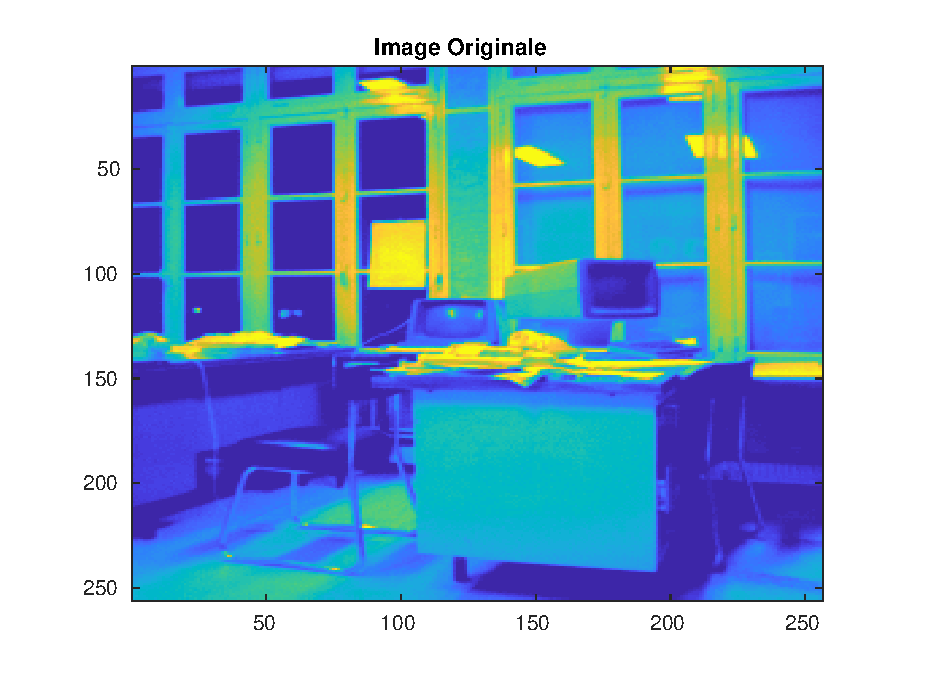
\includegraphics[width=0.3\textwidth]{Images/Matlab/imageOriginale}}};
    \end{tikzpicture} 
\end{figure}

\begin{figure}[H]
%\caption{}
    \begin{tikzpicture}[overlay]
    \node(a)[anchor=center, xshift=-3.2cm, yshift=2cm]{\centerline{\textbf{Récursif}}};
    \node(a)[anchor=center, xshift=3.3cm, yshift=2cm]{\centerline{\textbf{Convolutions}}};
    \node(a)[anchor=center, xshift=-4.85cm, yshift=0.2cm]{\centerline{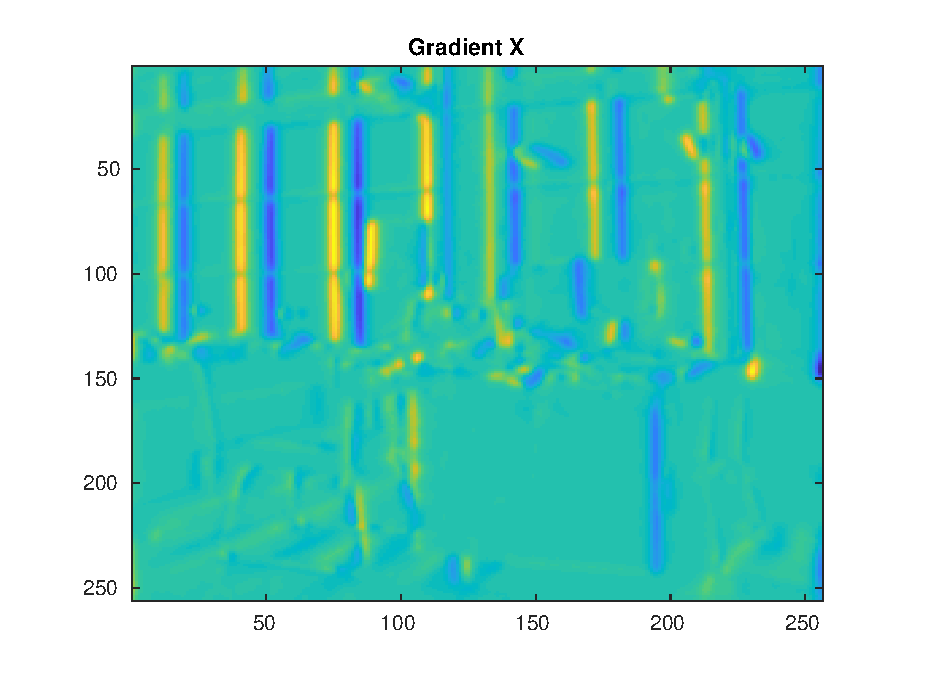
\includegraphics[width=0.29\textwidth]{Images/Matlab/ResultatsRecursif/gradientXrecursif}}};
    \node(a)[anchor=center, xshift=-1.55cm, yshift=0.2cm]{\centerline{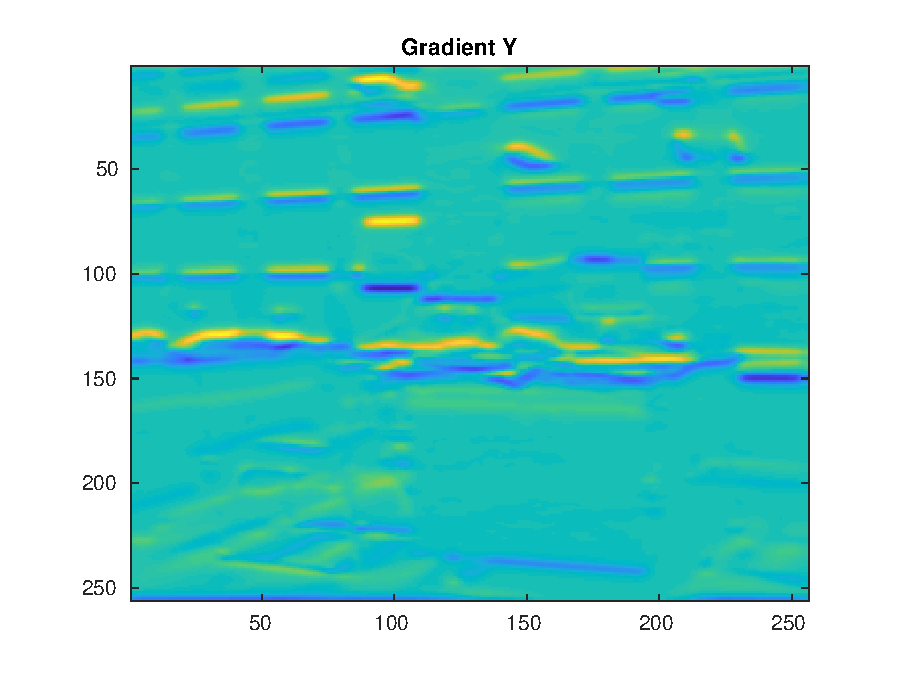
\includegraphics[width=0.29\textwidth]{Images/Matlab/ResultatsRecursif/gradientYrecursif}}};
    \node(a)[anchor=center, xshift=1.7cm, yshift=0.2cm]{\centerline{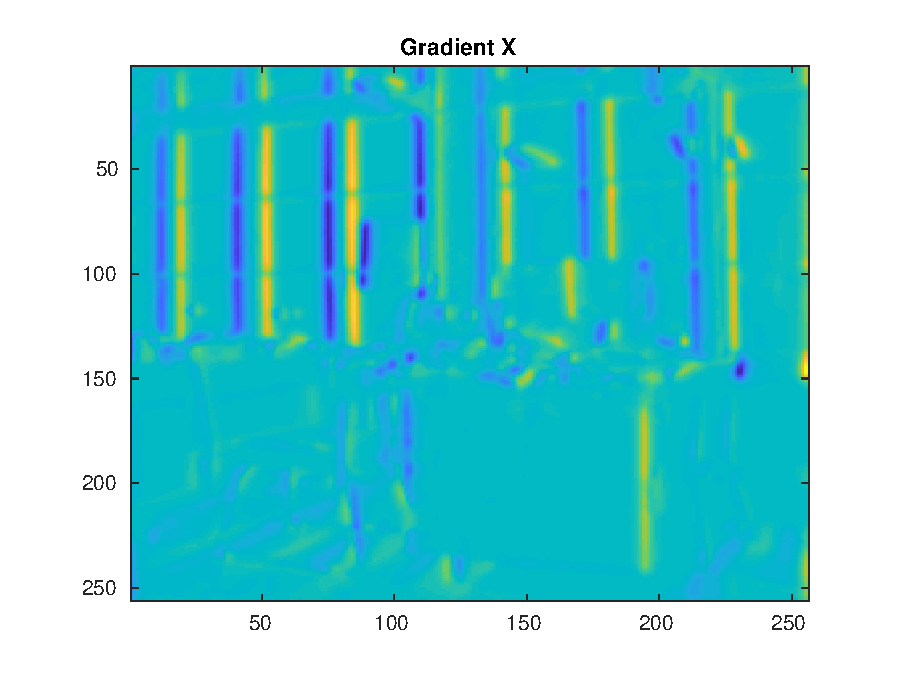
\includegraphics[width=0.29\textwidth]{Images/Matlab/ResultatsConvolutions/gradientXconvolutions}}};
    \node(a)[anchor=center, xshift=4.9cm, yshift=0.2cm]{\centerline{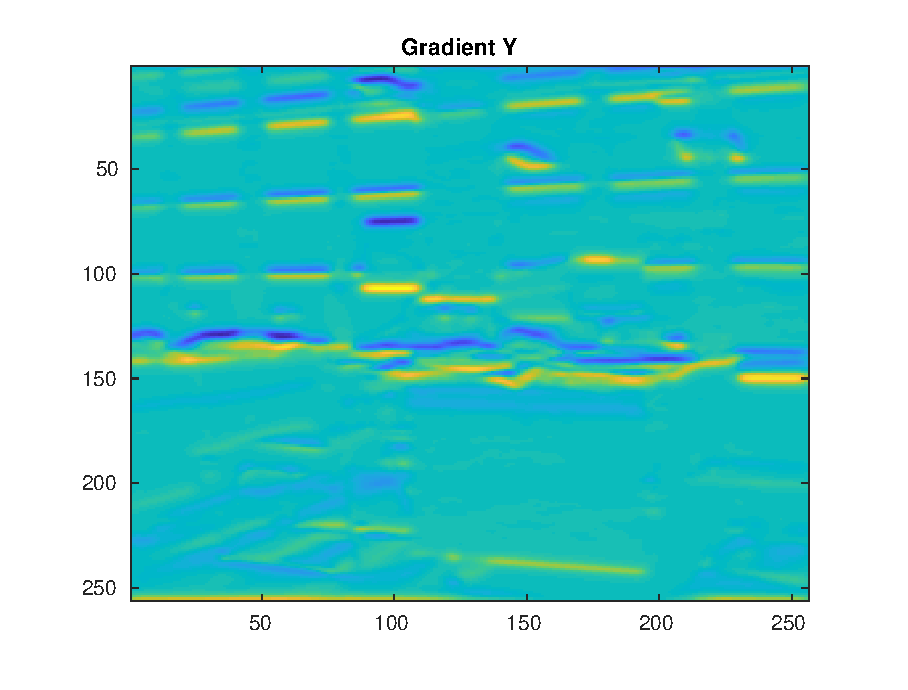
\includegraphics[width=0.29\textwidth]{Images/Matlab/ResultatsConvolutions/gradientYconvolutions}}};
    \node(a)[anchor=center, xshift=-4.85cm, yshift=-2.3cm]{\centerline{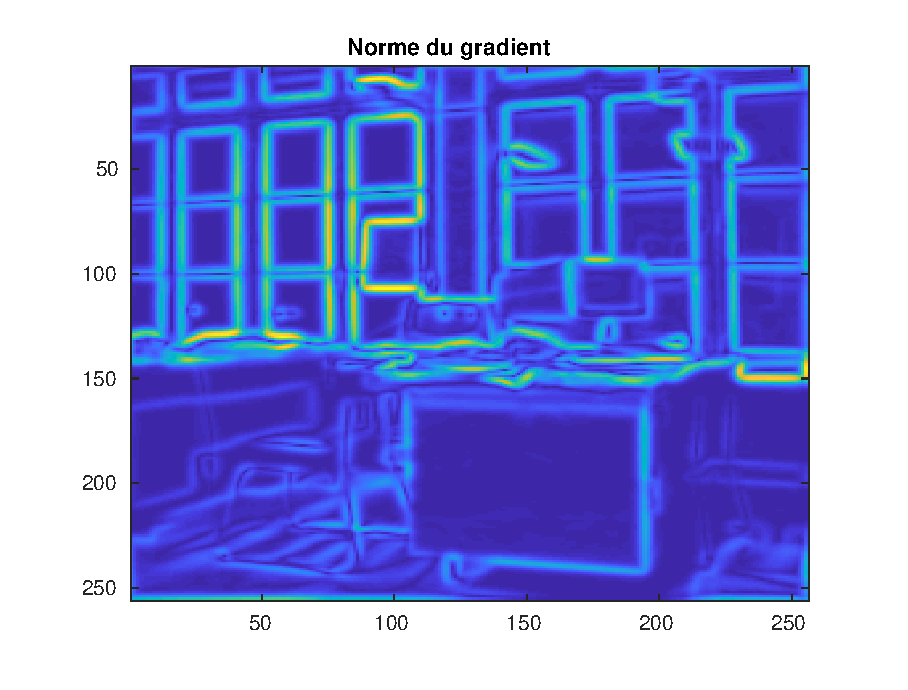
\includegraphics[width=0.29\textwidth]{Images/Matlab/ResultatsRecursif/normeGradientRecursif}}};
    \node(a)[anchor=center, xshift=-1.55cm, yshift=-2.3cm]{\centerline{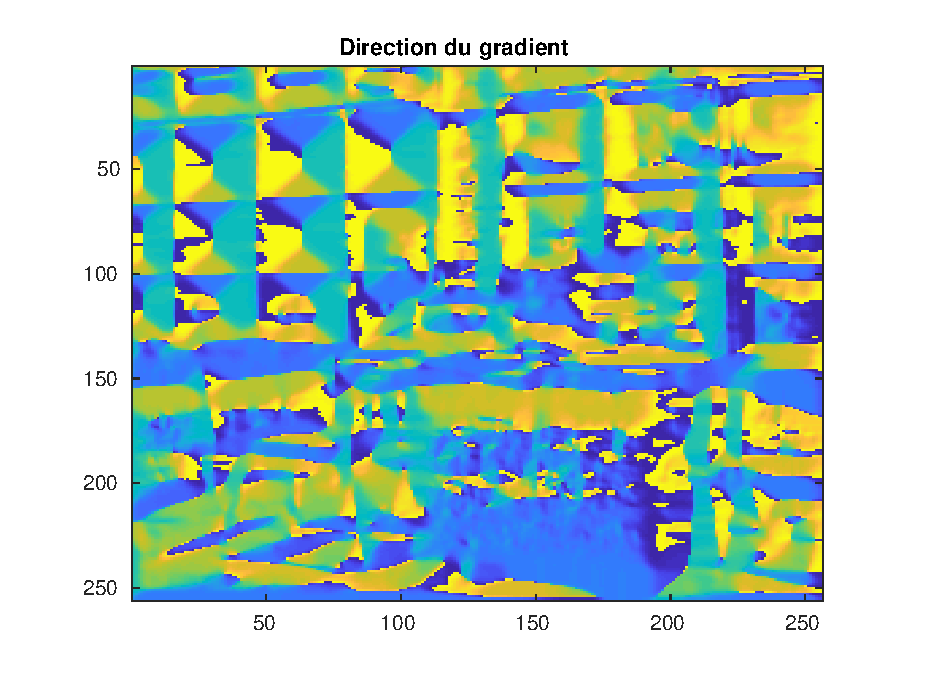
\includegraphics[width=0.29\textwidth]{Images/Matlab/ResultatsRecursif/directionGradientRecursif}}};
    \node(a)[anchor=center, xshift=1.7cm, yshift=-2.3cm]{\centerline{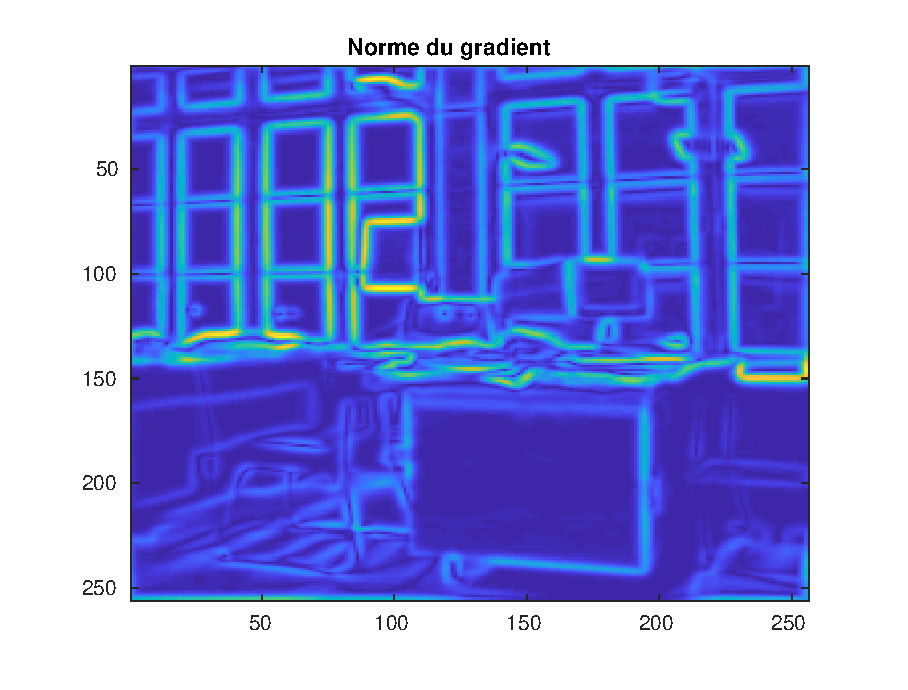
\includegraphics[width=0.29\textwidth]{Images/Matlab/ResultatsConvolutions/normeGradientConvolutions}}};
    \node(a)[anchor=center, xshift=4.9cm, yshift=-2.3cm]{\centerline{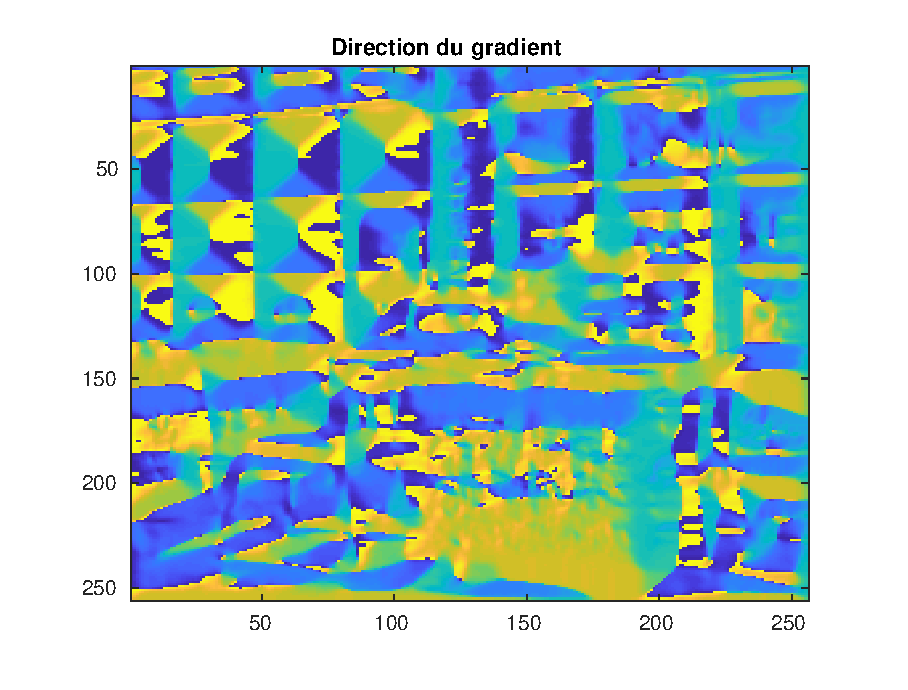
\includegraphics[width=0.29\textwidth]{Images/Matlab/ResultatsConvolutions/directionGradientConvolutions}}};
    \draw[-] (0.1cm,-3.8cm) -- (0.1cm,2cm) node[above,fill=none] {};
    \end{tikzpicture} 
\end{figure}

\end{frame}

\begin{frame}
\frametitle{Résultats}
% trim={<left> <lower> <right> <upper>}
\begin{figure}[H]
	\begin{tikzpicture}[overlay]
	\node(a)[anchor=center, xshift=0cm, yshift=3.2cm]{\centerline{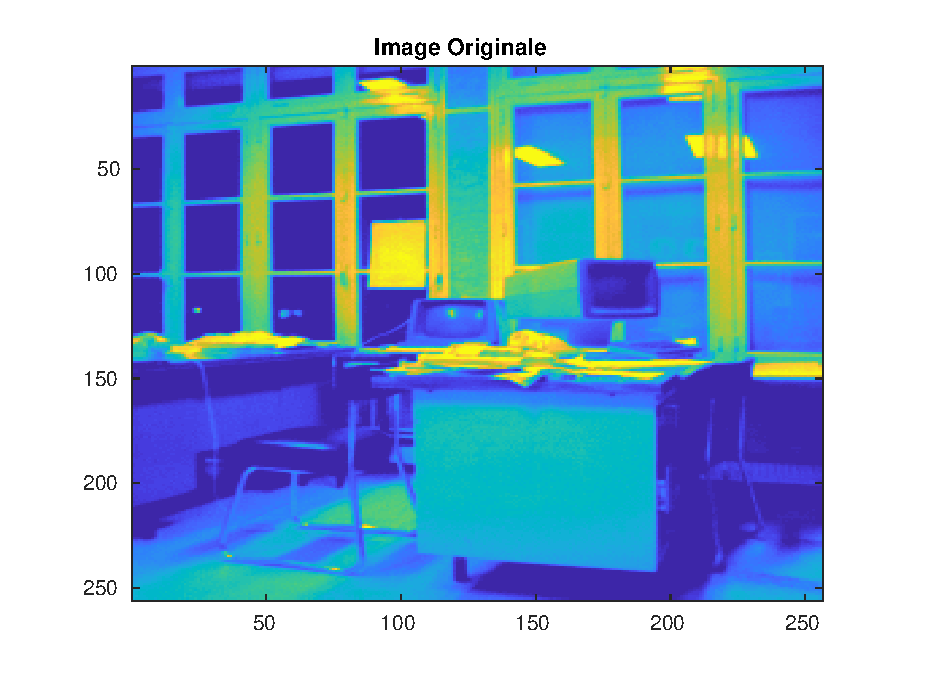
\includegraphics[width=0.3\textwidth]{Images/Matlab/imageOriginale}}};
	\node(a)[anchor=center, xshift=-3cm, yshift=2.3cm]{\centerline{\textbf{Récursif}}};
    \node(a)[anchor=center, xshift=3cm, yshift=2.3cm]{\centerline{\textbf{Convolutions}}};
 	\node(a)[anchor=center, xshift=-3cm, yshift=0.7cm]{\centerline{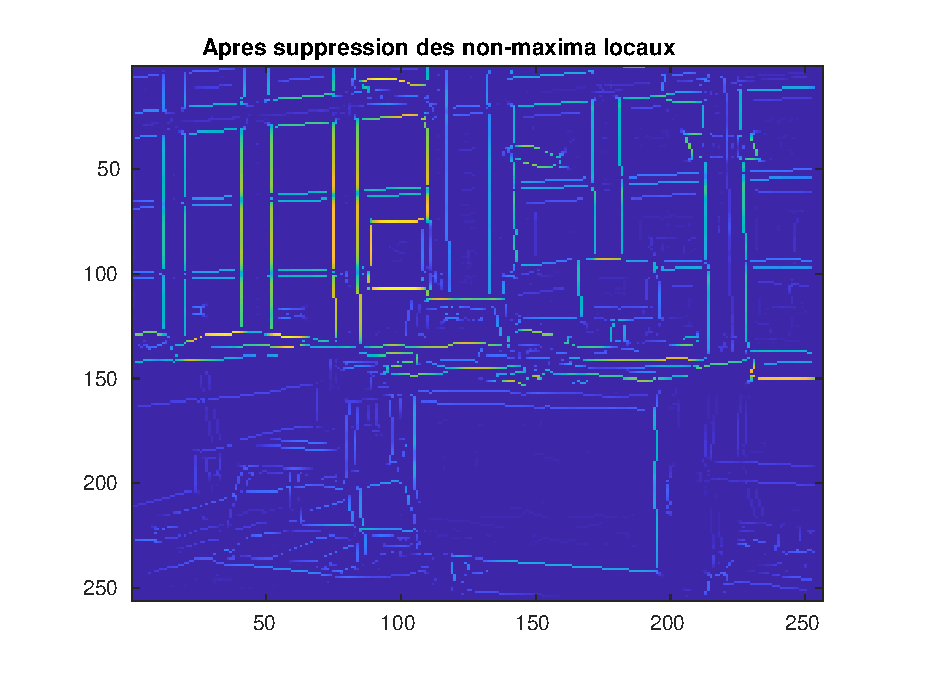
\includegraphics[width=0.29\textwidth]{Images/Matlab/ResultatsRecursif/suppnonmaxRecursif}}};
 	\node(a)[anchor=center, xshift=3cm, yshift=0.7cm]{\centerline{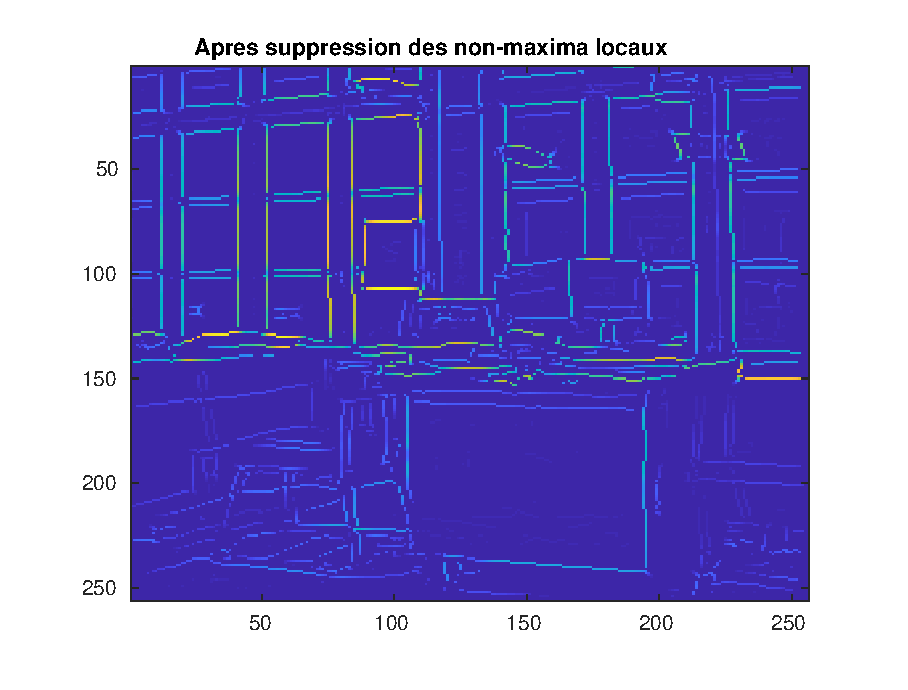
\includegraphics[width=0.29\textwidth]{Images/Matlab/ResultatsConvolutions/suppnonmaxConvolutions}}};
    \node(a)[anchor=center, xshift=-3cm, yshift=-2.8cm]{\centerline{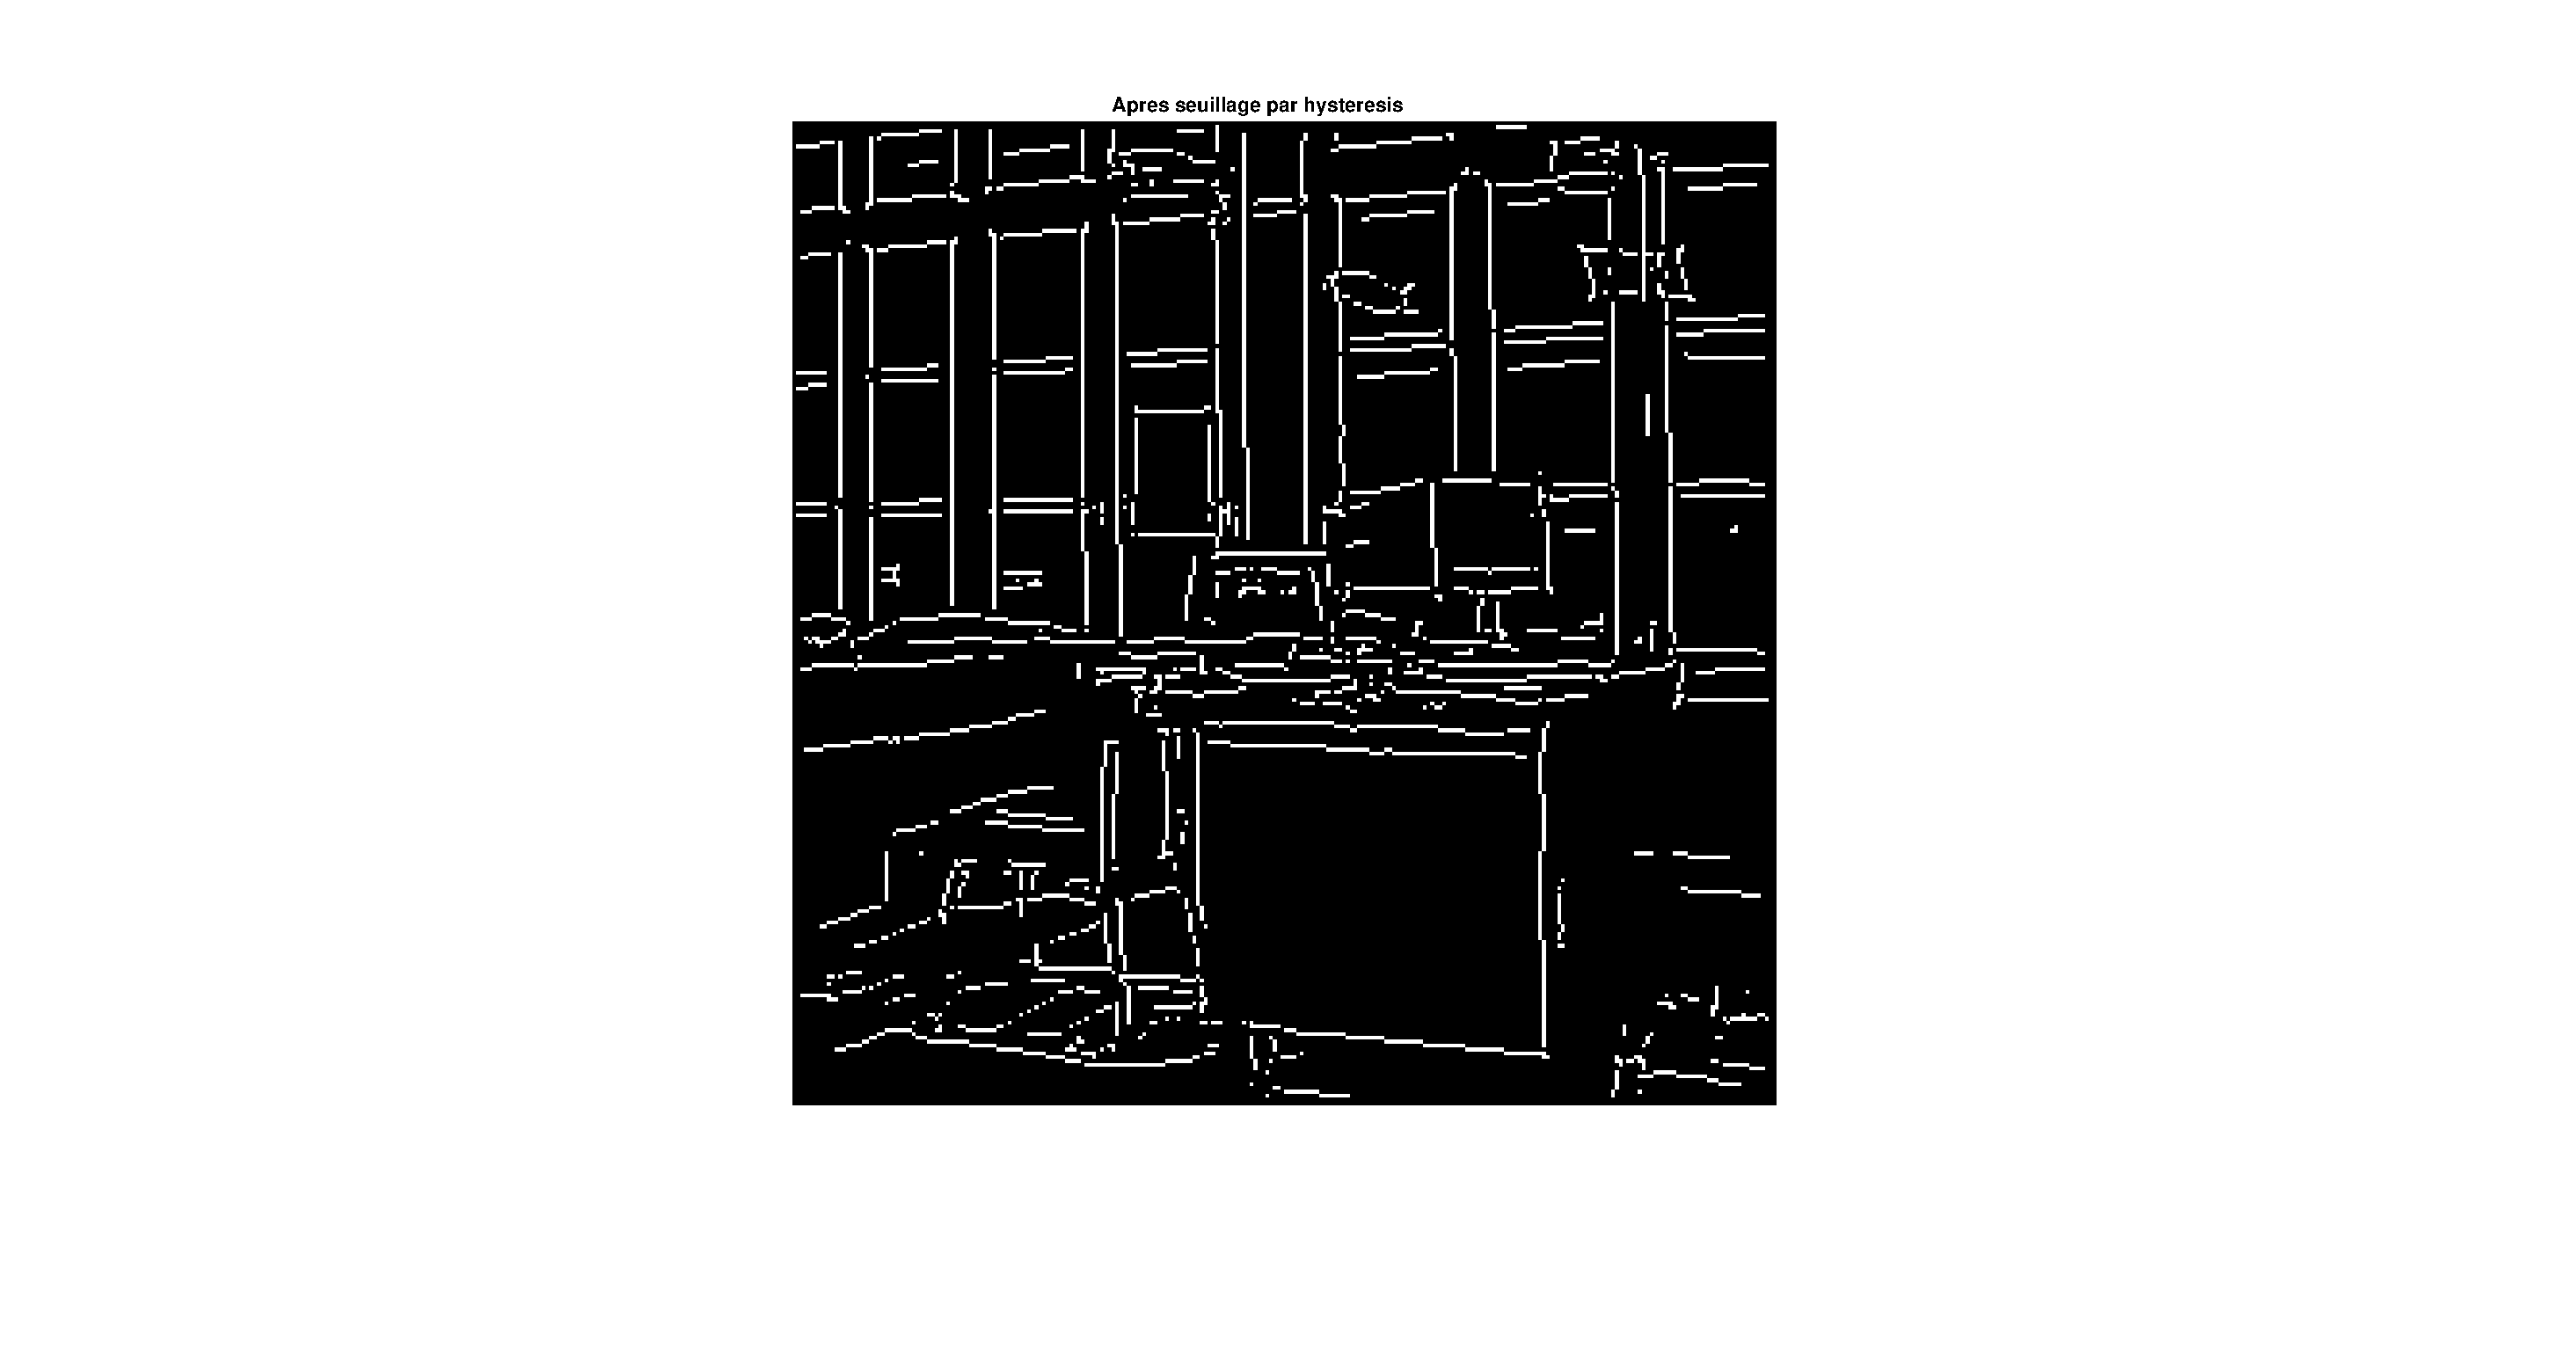
\includegraphics[trim={14.5cm 2cm 14.5cm 1cm},clip,width=0.35\textwidth]{Images/Matlab/ResultatsRecursif/resultatRecursif}}};    
    \node(a)[anchor=center, xshift=3cm, yshift=-2.8cm]{\centerline{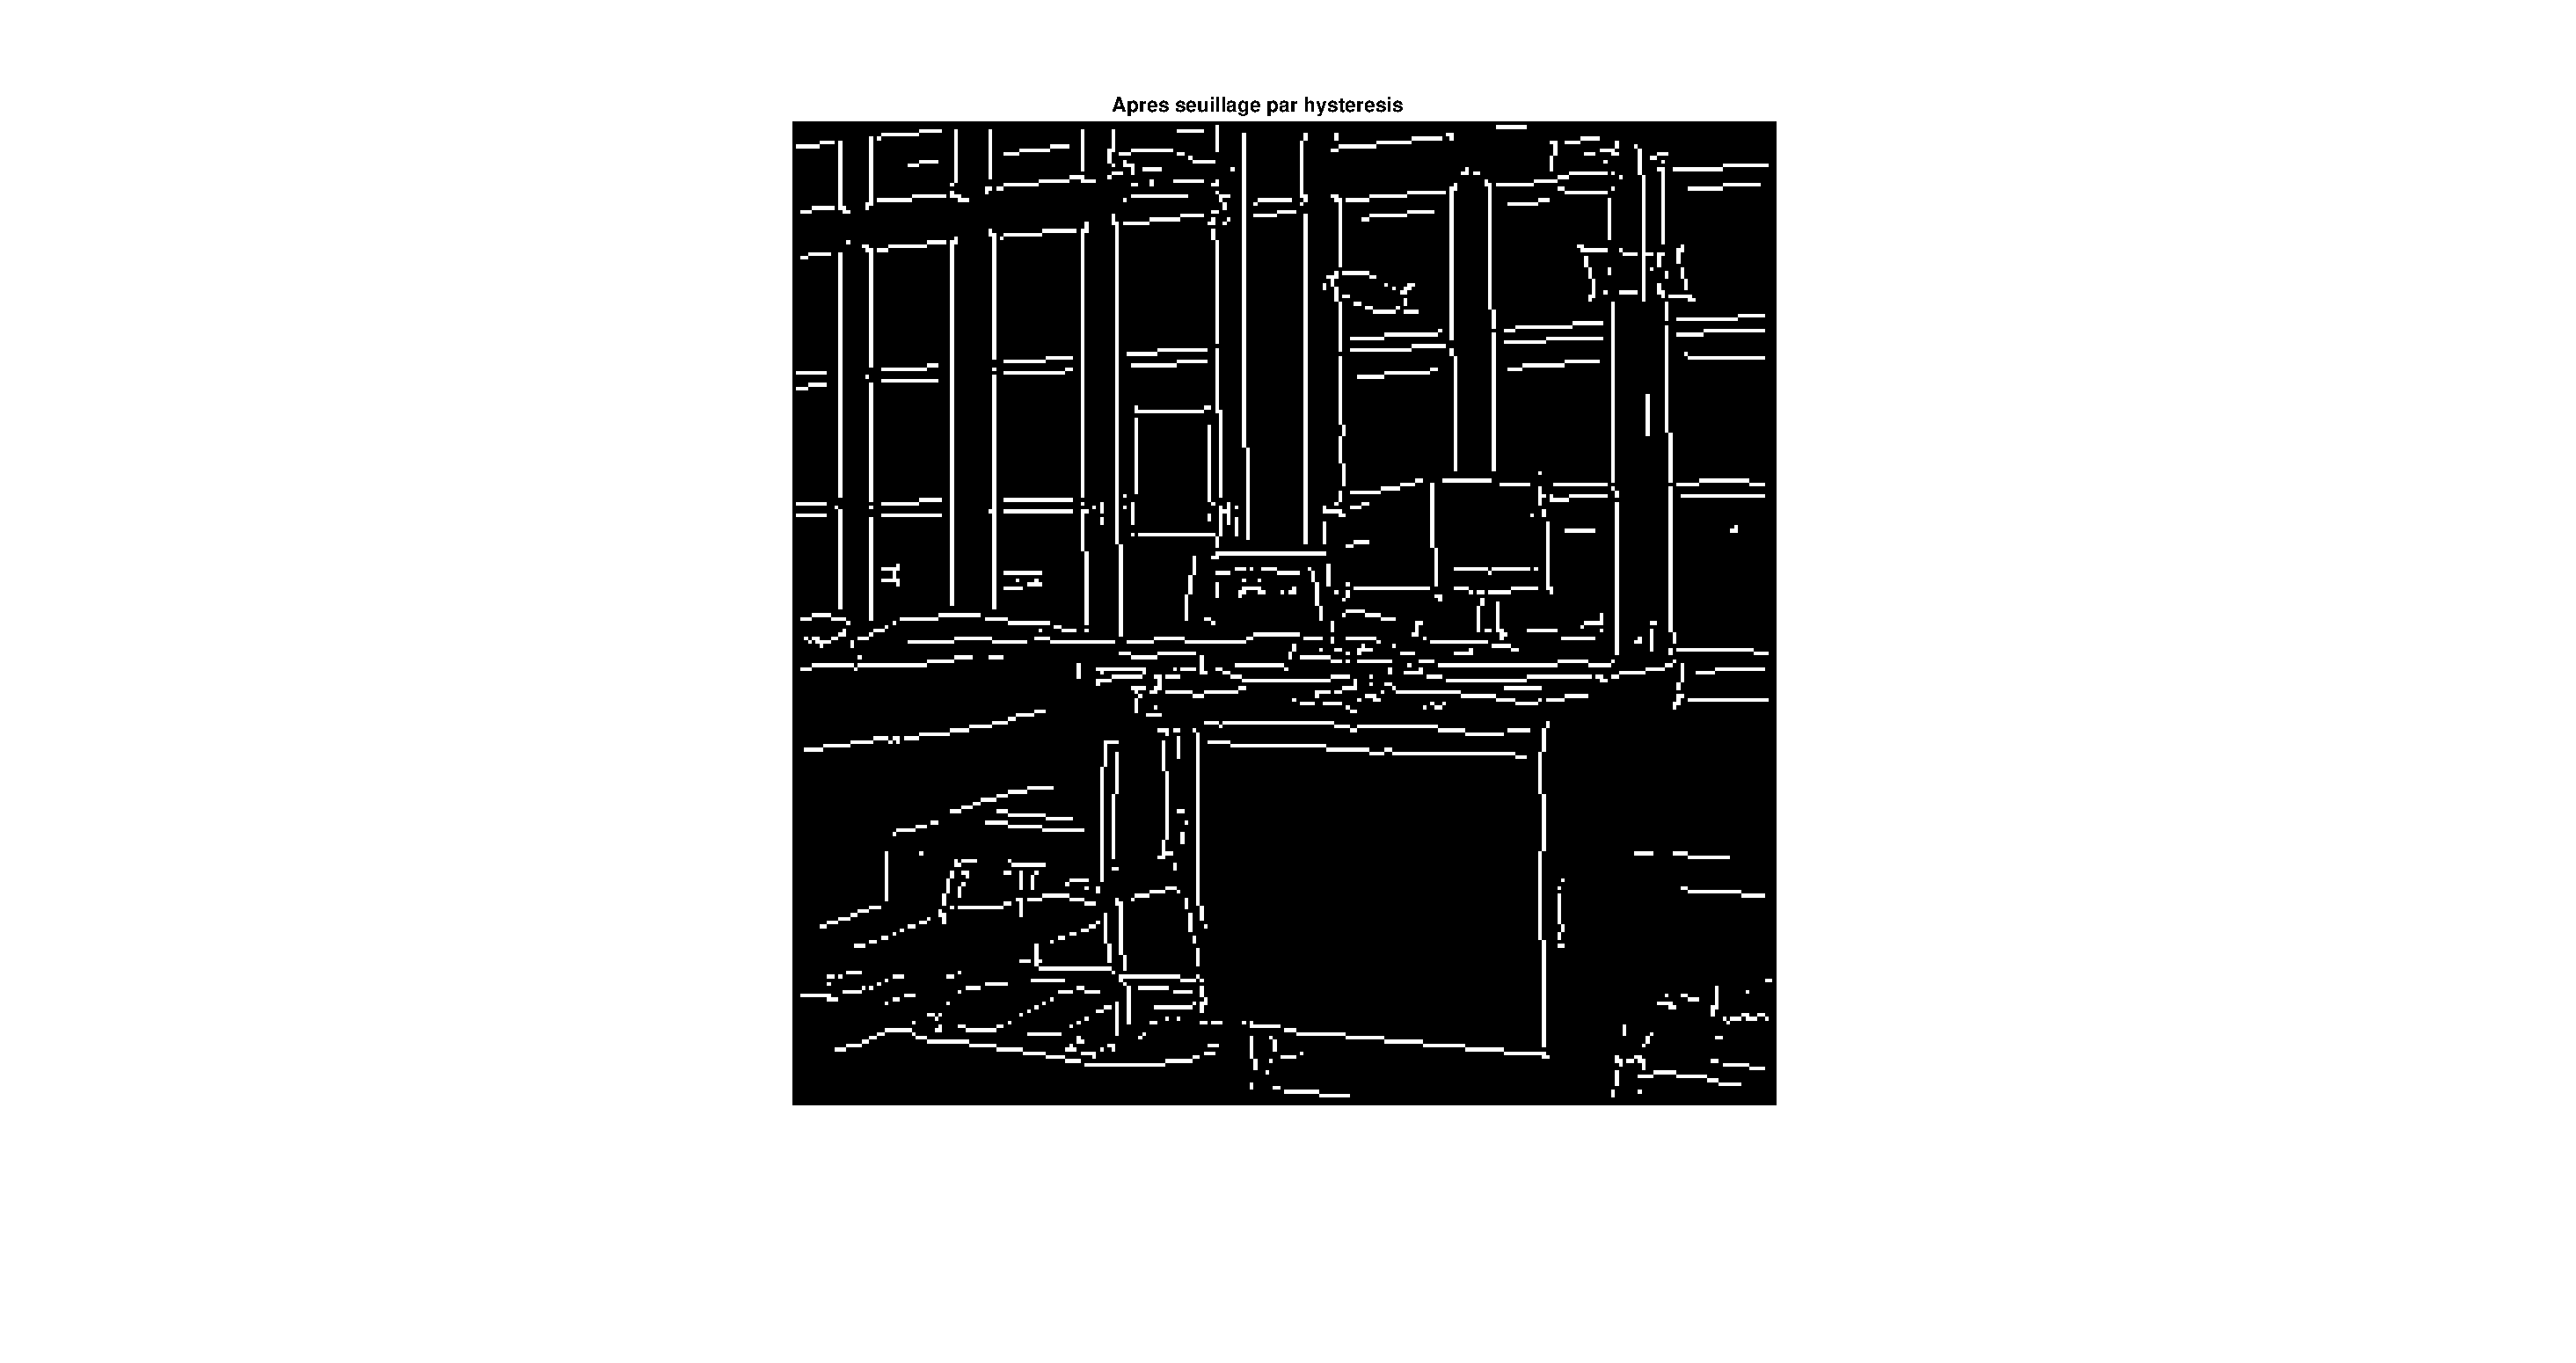
\includegraphics[trim={14.5cm 2cm 14.5cm 1cm},clip,width=0.35\textwidth]{Images/Matlab/ResultatsConvolutions/resultatConvolutions}}};
    \draw[-] (0.1cm,-4.4cm) -- (0.1cm,1.8cm) node[above,fill=none] {};
	\end{tikzpicture}
\end{figure}
\end{frame}

\begin{frame}
\frametitle{Résultats}
% trim={<left> <lower> <right> <upper>}
\begin{figure}[H]
	\begin{tikzpicture}[overlay]
	\node(a)[anchor=center, xshift=0cm, yshift=3.2cm]{\centerline{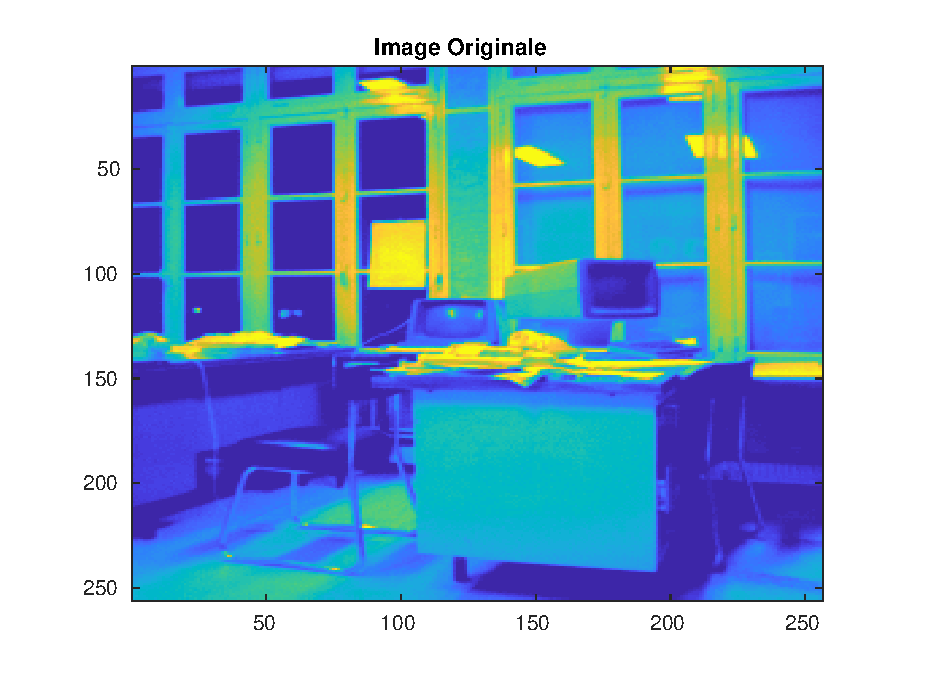
\includegraphics[width=0.3\textwidth]{Images/Matlab/imageOriginale}}};
	\node(a)[anchor=center, xshift=-3cm, yshift=2.7cm]{\centerline{\textbf{Récursif}}};
    \node(a)[anchor=center, xshift=3cm, yshift=2.7cm]{\centerline{\textbf{Convolutions}}};    
 	\node(a)[anchor=center, xshift=-3cm, yshift=0.6cm]{\centerline{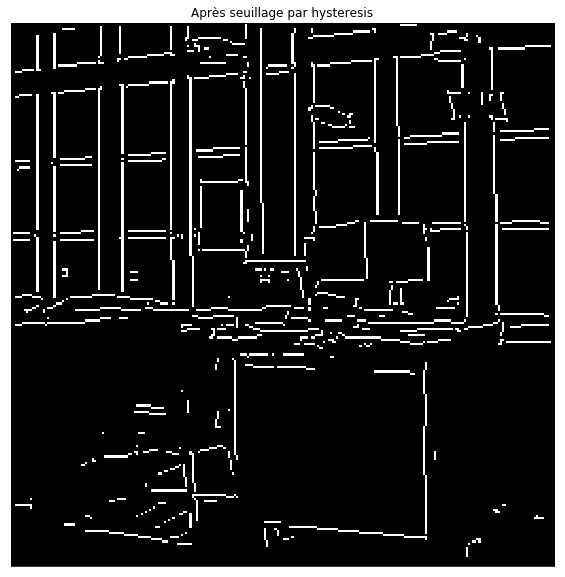
\includegraphics[width=0.3\textwidth]{Images/Python/resultatRecursif}}};
 	\node(a)[anchor=center, xshift=3cm, yshift=0.6cm]{\centerline{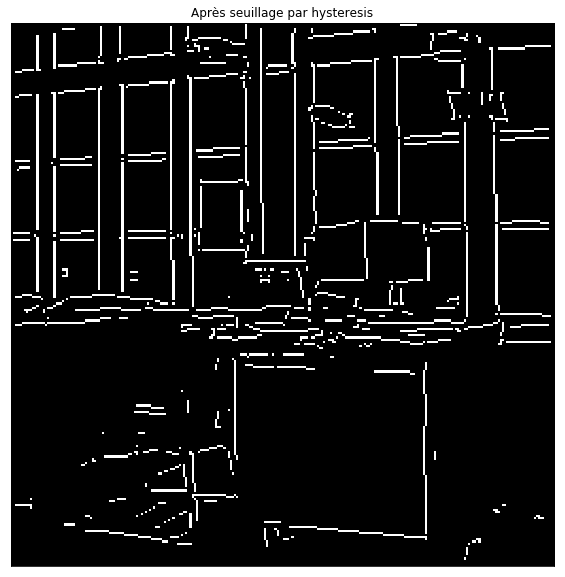
\includegraphics[width=0.3\textwidth]{Images/Python/resultatConvolutions}}};
    \node(a)[anchor=center, xshift=-3cm, yshift=-3.2cm]{\centerline{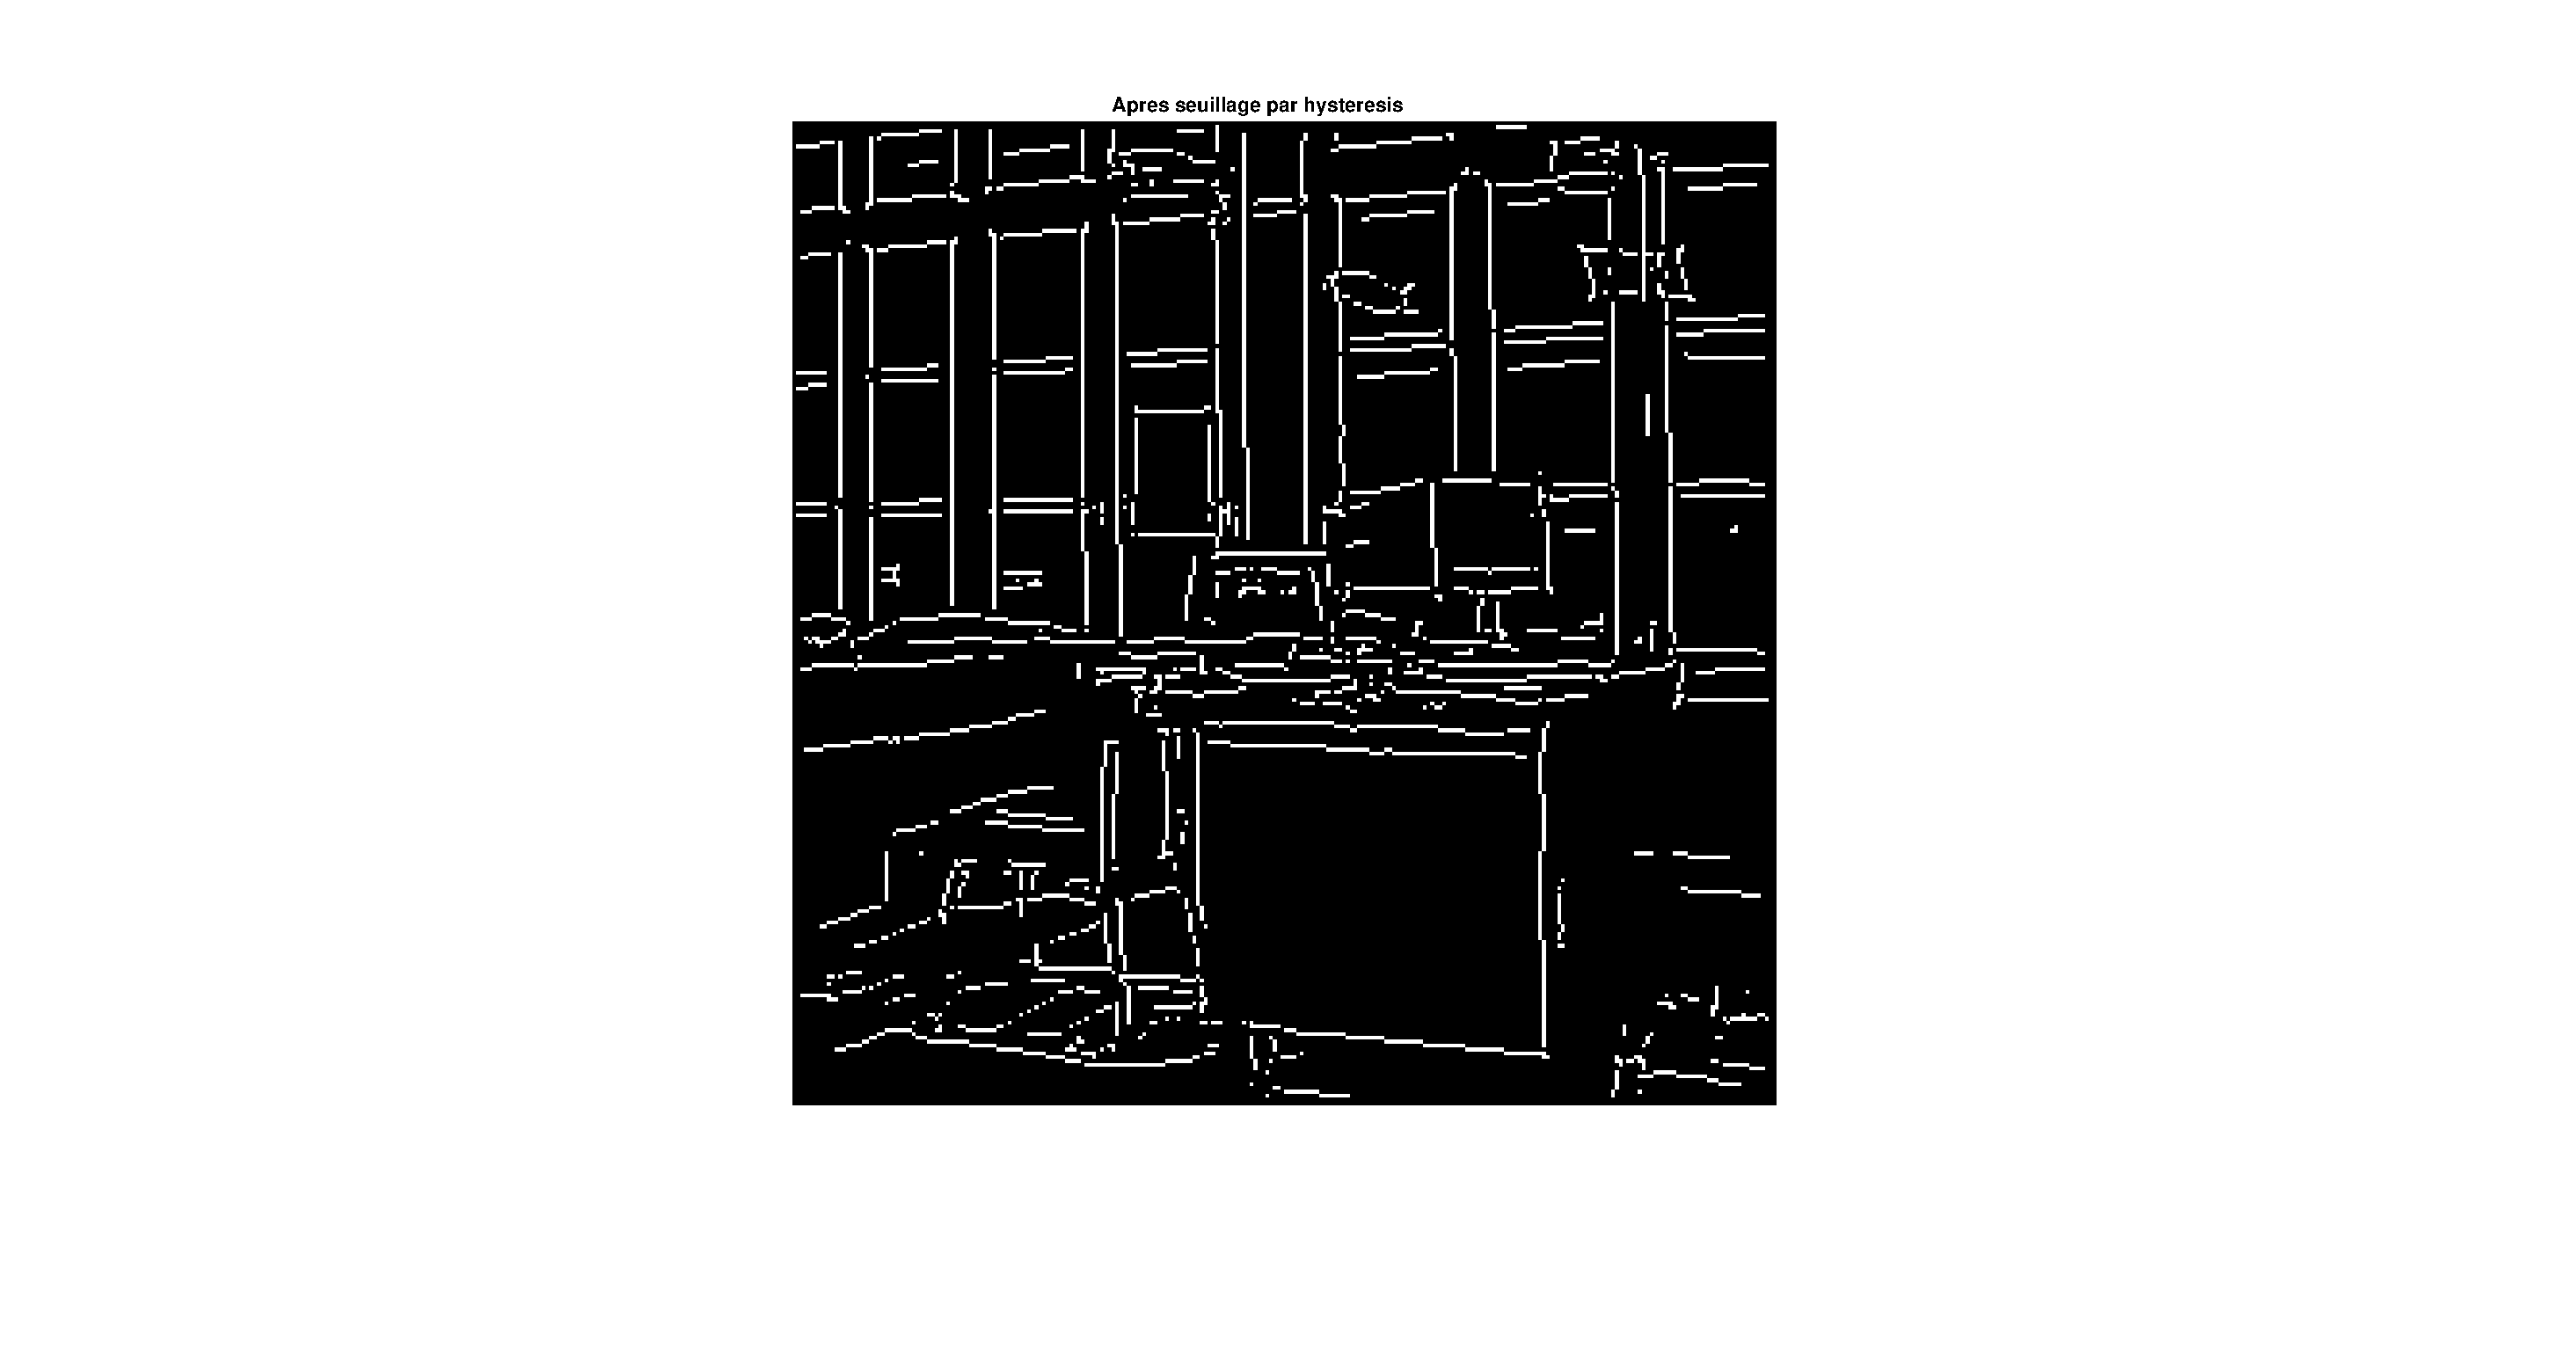
\includegraphics[trim={14.5cm 2cm 14.5cm 1cm},clip,width=0.3\textwidth]{Images/Matlab/ResultatsRecursif/resultatRecursif}}};    
    \node(a)[anchor=center, xshift=3cm, yshift=-3.2cm]{\centerline{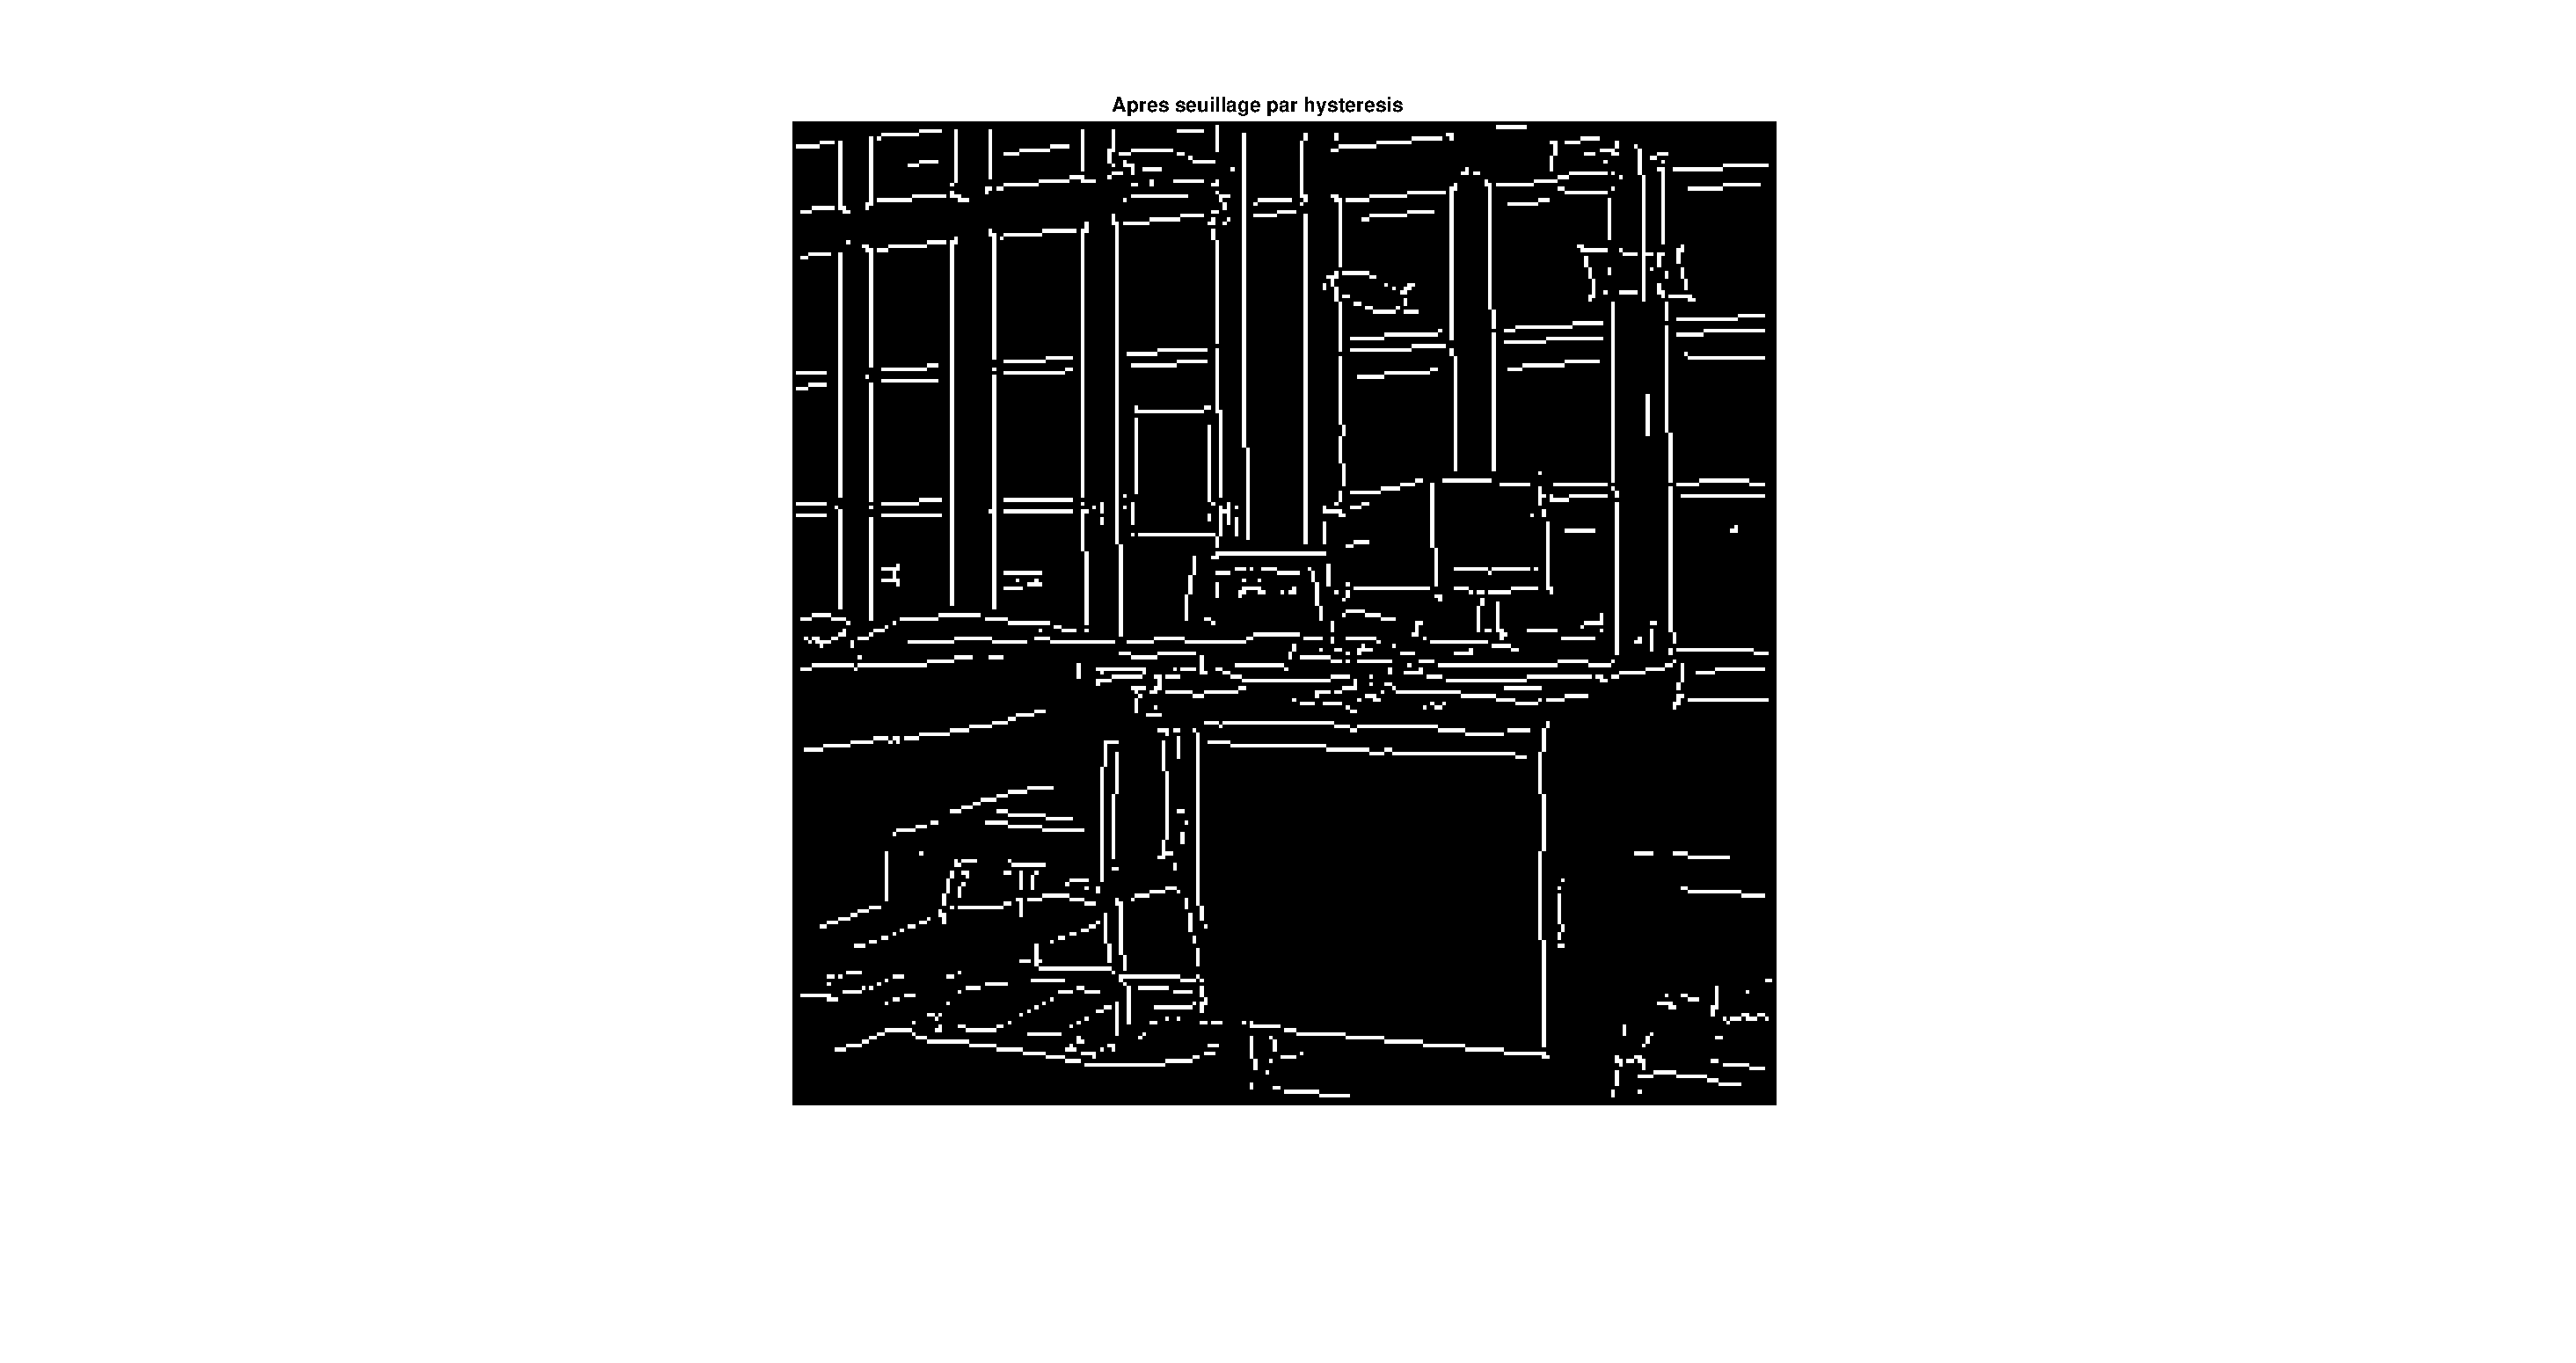
\includegraphics[trim={14.5cm 2cm 14.5cm 1cm},clip,width=0.3\textwidth]{Images/Matlab/ResultatsConvolutions/resultatConvolutions}}};
    \draw[-] (0.1cm,-4.4cm) -- (0.1cm,1.8cm) node[above,fill=none] {};
    \node(a)[anchor=center, xshift=-5.6cm, yshift=0.8cm]{\centerline{\textbf{Python}}};
    \node(a)[anchor=center, xshift=5.6cm, yshift=0.8cm]{\centerline{\textbf{Python}}};
    \node(a)[anchor=center, xshift=-5.6cm, yshift=-2.8cm]{\centerline{\textbf{Matlab}}};
    \node(a)[anchor=center, xshift=5.6cm, yshift=-2.8cm]{\centerline{\textbf{Matlab}}};
	\end{tikzpicture}
\end{figure}
\end{frame}

\section{Démonstrations}

\section{Bibliographie}
\begin{frame}
\frametitle{Bibliographie}
	
\begin{itemize}

\item[•] \textbf{\textcolor{magenta}{Article}}
\item[] \textbf{Titre} : Using Canny's Criteria to Derive a Recursively Implemented Optimal Edge
Detector
\item[] \textbf{Auteur} : RACHID DERICHE
\item[]

\item[•] Deriche edge detector
\item[] \url{https://en.wikipedia.org/wiki/Deriche_edge_detector} 

\item[•] Can't get clean output in my MATLAB implementation of Canny-Deriche
\item[] \url{https://stackoverflow.com/questions/14132356/cant-get-clean-output-in-my-matlab-implementation-of-canny-deriche} 

\item[•] Canny edge detector
\item[] \url{https://en.wikipedia.org/wiki/Canny_edge_detector} 

\item[•] Canny Edge Detection Step by step
\item[] \url{https://opencv-python-tutroals.readthedocs.io/en/latest/py_tutorials/py_imgproc/py_canny/py_canny.html} 

\end{itemize}
\end{frame}

\begin{frame}
\frametitle{Bibliographie}
	
\begin{itemize}
\item[•] Détection de contours : les opérateurs de Canny-Deriche
\item[] \url{https://perso.esiee.fr/~coupriem/Algo/algoima.html} 

\item[•] Extraction de contours et son extension du contour actif
\item[]
\url{http://ninebill.free.fr/ExtractionContours/detection/canny.html}

\item[•] JAVA demo of Canny/Deriche-like filter (EPFL Biomedical Imaging Group)
\item[] \url{http://bigwww.epfl.ch/demo/ip/demos/edgeDetector/} 

\item[•] Segmentator \--- Fix gramag export error with deriche filter (3D python)
\item[] \url{https://github.com/ofgulban/segmentator} 

\item[•] Edge Detection with MATLAB
\item[] \url{https://fr.mathworks.com/videos/edge-detection-with-matlab-119353.html} 

\item[•] Gaël Deest (pdf)
\item[] \url{www.theses.fr/2017REN1S102/abes} 
\end{itemize}
\end{frame}

\begin{frame}
\frametitle{Bibliographie}
	
\begin{itemize}

\item[•] Canny en python (OpenCV)
\item[] \url{https://opencv-python-tutroals.readthedocs.io/en/latest/py_tutorials/py_imgproc/py_canny/py_canny.html} 

\item[•] Convolution in Two Dimensions
\item[] \url{http://homepages.inf.ed.ac.uk/rbf/CVonline/LOCAL_COPIES/MARBLE/low/space/convol.htm} 

\item[•] Convolution en 2D
\item[] \url{http://web.stanford.edu/group/sequoia/cgi-bin/node/185} 

\item[•] EECS 442 \--- Computer vision
\item[] \url{http://vhosts.eecs.umich.edu/vision//teaching/EECS442_2012/lectures/lecture14.pdf} 

\item[•] DETECTION DE CONTOURS
\item[] \url{http://www.lirmm.fr/~strauss/PageImage3/EdgeDetection.pdf}
\end{itemize}
\end{frame}

\begin{frame}
\frametitle{Bibliographie}
	
\begin{itemize}
\item[•] Techniques d’extraction de contours
\item[] \url{ftp://ftp-sop.inria.fr/athena/Team/Rachid.Deriche/Lectures/Master-Stic-IGMMV/techniques_contours.pdf}

\item[•] Détection de contours
\item[] \url{http://devernay.free.fr/cours/vision/pdf/c3.pdf}

\item[•] Bases du traitement des images - Détection de contours
\item[] \url{http://webia.lip6.fr/~thomen/Teaching/BIMA/cours/contours.pdf}

\item[•] La détection decontours dans des images à niveaux de gris : mise en œuvre et sélection de détecteurs 
\item[] \url{http://docnum.univ-lorraine.fr/public/INPL_T_1991_ZIOU_D.pdf}

\item[•] Detection de contours
\item[] \url{http://dept-info.labri.fr/~achille/enseignement/TI/TI-ch4-notes.pdf}

\item[•] Segmentation d'image : Contours
\item[] \url{http://www.lgi2p.mines-ales.fr/~montesin/CoursPDF/segmentation_contours.pdf}

\item[•] Filtre de Deriche
\item[] \url{http://www.tsi.enst.fr/pages/enseignement/ressources/mti/Shen_ou_Deriche/node4.html}


\end{itemize}
\end{frame}

\end{document}